\documentclass[conference,a4paper]{IEEEtran}
% ------------------------------------------------------------------
% Urbanisation du SI du portail CNIE (DGSN) — rapport IEEE, français
% Compilation : latexmk -pdf main.tex   (MiKTeX, biber)
% ------------------------------------------------------------------
\usepackage[utf8]{inputenc}
\usepackage[T1]{fontenc}
\usepackage[french]{babel}
\usepackage{lmodern}
\usepackage{graphicx}
\usepackage{rotating}        % sidewaysfigure pour les BPMN
\usepackage{booktabs}
\usepackage{array}
\usepackage{tabularx}
\usepackage{xcolor}
\usepackage{enumitem}
\usepackage{caption}
\usepackage{subcaption}
\usepackage{microtype}
\usepackage{hyperref}
\usepackage[backend=biber,style=ieee,maxbibnames=3,sorting=none]{biblatex}
\addbibresource{biblio.bib}
\graphicspath{{figures/}}
\setlist{nosep}
\hypersetup{colorlinks=true,linkcolor=black,citecolor=blue!60!black,urlcolor=blue!60!black}
\definecolor{existant}{HTML}{E8D77A}
\definecolor{evoluer}{HTML}{F2B65C}
\definecolor{nouveau}{HTML}{7FCB8F}
\newcommand{\tagE}{\textcolor{existant}{\rule{0.9em}{0.9em}}}
\newcommand{\tagV}{\textcolor{evoluer}{\rule{0.9em}{0.9em}}}
\newcommand{\tagN}{\textcolor{nouveau}{\rule{0.9em}{0.9em}}}
\frenchbsetup{StandardLists=true}

\begin{document}

\title{Urbanisation du système d'information du portail de la Carte Nationale d'Identité Électronique~: cartographie de l'existant et architecture cible intégrant l'intelligence artificielle}

\author{%
\IEEEauthorblockN{Mouad, Najib, Hafsa, Zineb}
\IEEEauthorblockA{Cabinet d'urbanisation (projet académique) --- E-services dans l'administration marocaine, sujet~2\\
Novembre 2026}}

\maketitle

\begin{abstract}
La Direction Générale de la Sûreté Nationale (DGSN) délivre chaque année plusieurs millions de cartes nationales d'identité électroniques (CNIE) et opère, depuis 2022, la plateforme nationale d'identité numérique. Le portail \texttt{cnie.ma} dématérialise la pré-demande et la prise de rendez-vous, mais l'essentiel du contrôle des dossiers reste manuel et les canaux numériques de la DGSN demeurent cloisonnés. Ce rapport applique la démarche d'urbanisation des systèmes d'information au périmètre «~demande et renouvellement de la CNIE~». Il capte d'abord les orientations stratégiques de l'organisation (Digital Morocco 2030, loi 55-19, lutte contre la fraude, inclusion), puis décline le système cible en quatre cartographies cohérentes~: métier (processus principal modélisé en BPMN sous IBM Blueworks Live, dans ses versions actuelle et cible), fonctionnelle (plan d'occupation des sols distinguant blocs existants, à faire évoluer et nouveaux), applicative (quinze composants cibles et leurs flux) et technique (architecture en zones, cloud souverain, PKI, plateforme d'inférence). Cinq cas d'usage d'intelligence artificielle sont intégrés au cœur du processus~: assistant conversationnel, contrôle documentaire automatique, vérification biométrique anti-fraude, prévision d'affluence et détection d'anomalies. Le sous-processus de pré-demande, de contrôle des pièces et de prise de rendez-vous a été prototypé sous Bonitasoft pour valider l'orchestration et les interfaces. Une trajectoire en trois paliers (2027, 2028, 2030) et un dispositif de gouvernance complètent la proposition.
\end{abstract}

\begin{IEEEkeywords}
urbanisation des SI, architecture d'entreprise, ArchiMate, BPMN, identité numérique, CNIE, DGSN, intelligence artificielle, e-gouvernement, Bonita, Blueworks Live
\end{IEEEkeywords}

\section{Introduction}

\subsection{Contexte}
La carte nationale d'identité électronique est le titre régalien le plus diffusé du Royaume~: la génération lancée en août 2020 équipait déjà quinze millions de citoyens en 2023, soit environ 85~\% de la population de plus de seize ans \cite{dgsn2023tcn}, et la DGSN a produit près de 3,7 millions de cartes au cours de la seule année 2025 \cite{lavieeco2025bilan}. Au-delà du support physique, la loi 04-20 a fait de la CNIE un titre certifiant l'identité numérique de son porteur \cite{loi0420}. Sur cette base, la DGSN et l'Agence de Développement du Digital ont ouvert en avril 2022 la plateforme «~Tiers de Confiance National~», qui permet à des fournisseurs de services accrédités de déléguer l'identification et l'authentification de leurs usagers \cite{lavieeco2022tcn}. Plus de trente organismes publics et privés y étaient raccordés fin 2024 \cite{allafrica2024bilan}, et le portail \texttt{epolice.ma}, lancé en décembre 2024, s'appuie sur elle pour délivrer la fiche anthropométrique à distance \cite{telquel2024epolice}.

Le portail \texttt{cnie.ma}, objet de cette étude, constitue le point d'entrée du processus d'obtention et de renouvellement de la carte~: depuis septembre 2020, la pré-demande et la prise de rendez-vous en ligne y sont obligatoires avant tout passage en centre d'enregistrement \cite{telquel2020rdv}. Ce dispositif a absorbé une forte montée en charge, mais il reste un portail de «~première génération~»~: il collecte des données puis renvoie le citoyen vers un parcours physique largement manuel.

\subsection{Problématique et commande}
Les décideurs de la DGSN souhaitent faire évoluer ce système pour le rendre plus efficace, plus réactif et plus personnalisé, en y intégrant des outils d'intelligence artificielle. Dans le rôle du cabinet d'urbanisation mandaté, nous devons~: (i)~étudier et cartographier l'existant, (ii)~proposer le système cible en nous appuyant sur l'existant, sur les standards d'architecture d'entreprise et sur les bonnes pratiques du domaine de l'identité numérique.

La question centrale est donc la suivante~: \emph{comment réorganiser le système d'information du périmètre CNIE pour que le parcours du citoyen devienne majoritairement numérique, que la fraude soit détectée au plus tôt, que la capacité des centres soit pilotée par la donnée, tout en respectant les exigences de souveraineté et de protection des données personnelles~?}

\subsection{Périmètre et choix structurants}
Le processus principal retenu est \textbf{P0 -- Demande et renouvellement de la CNIE}, de l'expression du besoin jusqu'à la remise de la carte et l'activation de l'identité numérique. Il concentre l'essentiel des volumes, des irritants et des opportunités d'automatisation. Le sous-processus \textbf{SP1 -- Pré-demande en ligne, contrôle des pièces et prise de rendez-vous} a été choisi pour le prototypage sous Bonitasoft, car il est celui où l'intelligence artificielle transforme le plus directement l'expérience du citoyen.

\subsection{Organisation du rapport}
La section~\ref{sec:methodo} présente la démarche d'urbanisation et les outils employés. La section~\ref{sec:existant} cartographie l'existant et en dresse le diagnostic. La section~\ref{sec:strategie} capte la stratégie et les cas d'usage d'intelligence artificielle. Les sections~\ref{sec:metier} à~\ref{sec:technique} déclinent les cartographies métier, fonctionnelle, applicative (avec le prototype Bonita) et technique du système cible. La section~\ref{sec:trajectoire} propose la trajectoire de migration et la gouvernance, avant la conclusion.

\section{Cadre méthodologique}
\label{sec:methodo}

\subsection{L'urbanisation des systèmes d'information}
L'urbanisation applique au système d'information les principes d'aménagement d'une ville~: on découpe le territoire en zones, quartiers, îlots et blocs aux responsabilités claires, on fixe des règles de voirie (les échanges) et l'on fait évoluer le bâti progressivement, sans tout raser \cite{longepe2009, club_urba2010}. La démarche s'organise en quatre couches qui se répondent~: la couche \emph{métier} (stratégie, processus, acteurs), la couche \emph{fonctionnelle} (ce que le SI doit savoir faire, indépendamment des logiciels), la couche \emph{applicative} (les logiciels qui portent ces fonctions et leurs flux) et la couche \emph{technique} (les infrastructures d'exécution). L'alignement des quatre couches, de la stratégie vers la technique, constitue le fil conducteur de ce rapport.

Pour chaque couche nous distinguons l'\emph{existant} (\emph{as-is}) et la \emph{cible} (\emph{to-be}), puis nous qualifions chaque bloc selon trois statuts, repris dans toutes les figures~: \tagE~existant conservé, \tagV~existant à faire évoluer, \tagN~nouveau.

\subsection{Standards et notations}
Nous utilisons trois standards complémentaires. \textbf{ArchiMate 3.2} \cite{archimate32} fournit un langage unique pour relier motivations, stratégie, métier, applications, technologie et trajectoire de migration~; il garantit la cohérence entre nos cartographies et a été outillé avec Archi \cite{archi_tool}. \textbf{BPMN 2.0} \cite{bpmn20} sert à modéliser le processus principal avec ses couloirs d'acteurs, ses passerelles de décision et ses événements~; les modèles ont été construits sous IBM Blueworks Live \cite{blueworks_doc}. Enfin, la méthode \textbf{TOGAF} \cite{togaf10} inspire l'enchaînement vision, architectures, opportunités et solutions, planification de la migration, que nous avons adapté au format demandé.

\subsection{Démarche suivie}
Le travail s'est déroulé en cinq étapes~:
\begin{enumerate}
  \item \emph{Étude de l'existant}~: analyse du parcours proposé par \texttt{cnie.ma}, des portails connexes (\texttt{epolice.ma}, \texttt{identitenumerique.ma}), de la documentation publique de la DGSN et de la presse spécialisée~; reconstitution des cartographies actuelles.
  \item \emph{Captation de la stratégie}~: entretien simulé avec les décideurs à partir des orientations nationales et des bilans annuels de l'organisation~; formalisation en vue de motivation ArchiMate.
  \item \emph{Conception de la cible}~: processus cible en BPMN, plan d'occupation des sols fonctionnel, cartographie applicative, architecture technique.
  \item \emph{Prototypage}~: implémentation du sous-processus SP1 sous Bonita Studio \cite{bonita_doc} (modèle de données, formulaires, règles de décision, simulation du service d'IA).
  \item \emph{Trajectoire}~: découpage en paliers, chantiers, gouvernance et risques.
\end{enumerate}

\subsection{Outils}
\begin{table}[h]
\caption{Outils mobilisés par livrable}
\label{tab:outils}
\centering
\small
\begin{tabularx}{\columnwidth}{lX}
\toprule
\textbf{Livrable} & \textbf{Outil} \\
\midrule
Stratégie, cartographies fonctionnelle, applicative, technique, trajectoire & Archi (ArchiMate 3.2) \\
Processus métier actuel et cible & IBM Blueworks Live (BPMN 2.0) \\
Interfaces du sous-processus SP1 & Bonita Studio Community (BPM, BDM, UI Designer) \\
Rédaction & \LaTeX{} (classe IEEEtran) \\
\bottomrule
\end{tabularx}
\end{table}

\section{Étude et cartographie de l'existant}
\label{sec:existant}

\subsection{L'organisation et son écosystème}
La DGSN, rattachée au Ministère de l'Intérieur, est l'autorité de délivrance de la CNIE. Elle s'appuie sur un réseau de centres d'enregistrement des données identitaires (CEDI) répartis sur le territoire, sur deux centres de production (Rabat et Marrakech) qui ont personnalisé respectivement 2,65 et plus d'un million de cartes en 2025 \cite{lavieeco2025bilan}, et sur les services consulaires pour les Marocains résidant à l'étranger. Autour d'elle gravitent l'Agence de Développement du Digital (promotion et support de l'identité numérique), la CNDP (protection des données), la DGSSI (sécurité des systèmes), la Trésorerie Générale pour l'e-timbre, et les fournisseurs de services accrédités à la plateforme Tiers de Confiance National.

\subsection{Les e-services actuels}
Le portail \texttt{cnie.ma} offre quatre fonctions principales \cite{infopratique2026, wadifa2026}~:
\begin{itemize}
  \item la \textbf{pré-demande}, qui recueille le type de demande (première délivrance, renouvellement, duplicata), l'identité en caractères latins et arabes, l'état civil et la filiation, l'adresse de résidence, les coordonnées et un contact d'urgence facultatif destiné à la puce~;
  \item la \textbf{prise de rendez-vous} dans un CEDI, par date et créneau, modifiable ou annulable~;
  \item le \textbf{suivi de la demande} par numéro, avec six statuts (pré-demande, en cours, disponible, remise, dossier incomplet, annulée)~;
  \item des services annexes~: demande de code PIN, prise en charge des cas particuliers (personnes alitées ou handicapées) et information sur les pièces à fournir.
\end{itemize}
Le paiement s'effectue par e-timbre de 75~DH (50~DH avant douze ans), acheté auprès des canaux agréés. La carte est valable dix ans pour les adultes.

À côté de ce portail, la DGSN exploite \texttt{identitenumerique.ma} et l'application «~Mon identité numérique~», qui permettent au porteur d'activer son identité dérivée de la carte, de gérer ses consentements et ses moyens d'authentification, et d'être alerté à chaque usage \cite{dgsn2023tcn}~; ainsi que \texttt{epolice.ma}, qui regroupe depuis fin 2024 des téléservices de police \cite{telquel2024epolice}.

\subsection{Le processus actuel}
La figure~\ref{fig:bpmn-asis} modélise le processus actuel tel que vécu par le citoyen. Trois ruptures de canal le caractérisent~: la pré-demande numérique se termine par l'impression et la signature d'un formulaire papier~; le contrôle des pièces n'intervient qu'au guichet, si bien qu'un dossier incomplet se solde par un nouveau rendez-vous~; enfin, le retrait exige un second déplacement, et l'activation de l'identité numérique relève d'une démarche séparée.

\begin{sidewaysfigure*}
\centering
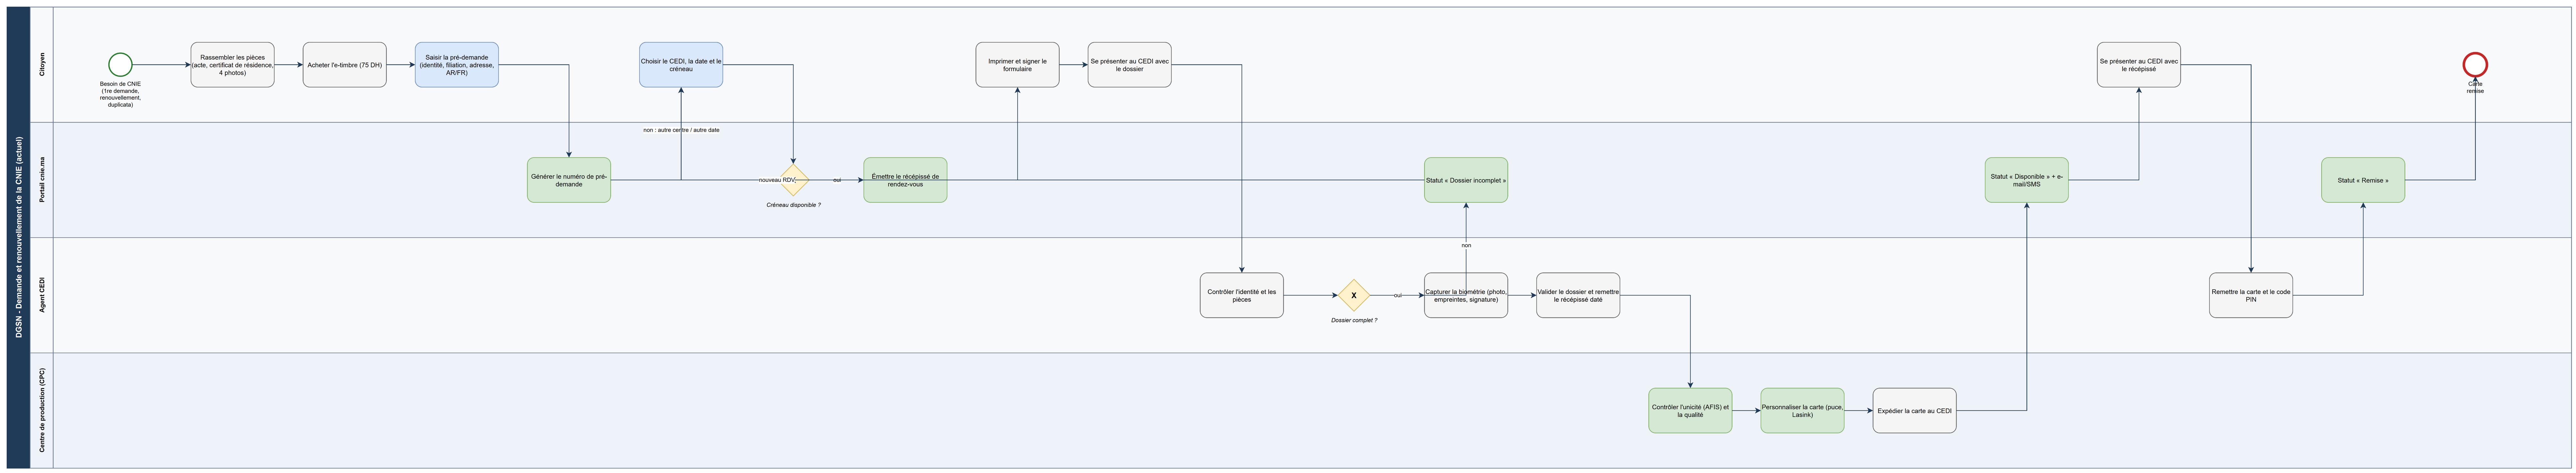
\includegraphics[width=\textwidth]{bpmn/P0_demande_cnie_asis.png}
\caption{Processus P0 actuel (as-is)~: demande et renouvellement de la CNIE. Bleu~: tâches utilisateur sur le portail~; gris~: tâches manuelles~; vert~: tâches automatiques.}
\label{fig:bpmn-asis}
\end{sidewaysfigure*}

\subsection{Cartographies de l'existant}
\paragraph{Fonctionnel} Le SI actuel couvre les fonctions de pré-demande, de rendez-vous, de suivi, d'enrôlement biométrique, de production, de gestion du cycle de vie de la carte (révocation, PIN) et d'identité numérique. Il ne couvre pas, ou seulement manuellement, le contrôle documentaire, l'instruction à distance, la gestion des réclamations, la prévision de charge et le pilotage.
\paragraph{Applicatif} On identifie un portail web, un système de rendez-vous, les postes d'enrôlement des CEDI reliés au référentiel biométrique (AFIS/ABIS), le système de production et de personnalisation, la plateforme Tiers de Confiance National et ses kits hors-ligne, et des échanges ponctuels avec l'e-timbre et les consulats. Les portails sont développés et exploités séparément.
\paragraph{Technique} La plateforme d'identité est décrite par la DGSN comme un système souverain, hébergé et opéré en interne, fondé sur la lecture NFC de la puce, le PIN et la biométrie, et exposé aux partenaires via OpenID Connect \cite{dgsn2023tcn, oidc}.

\subsection{Diagnostic}
\begin{table}[h]
\caption{Synthèse du diagnostic de l'existant}
\label{tab:diag}
\centering
\small
\begin{tabularx}{\columnwidth}{lX}
\toprule
\textbf{Forces} & Couverture nationale quasi complète de la CNIE~2~; rendez-vous en ligne généralisé~; plateforme d'identité numérique souveraine, sans registre central, déjà adoptée par plus de trente partenaires~; capacités de production éprouvées. \\
\midrule
\textbf{Faiblesses} & Contrôle des pièces manuel et tardif~; double saisie (portail puis papier)~; statuts de suivi grossiers, pas de délai annoncé~; renouvellement aussi lourd qu'une première demande malgré une biométrie déjà connue~; canaux et portails en silos. \\
\midrule
\textbf{Opportunités} & Digital Morocco 2030 et loi 55-19~; maturité de l'OCR, de la vision par ordinateur et des modèles de langue~; application mobile d'identité comme futur canal unique~; données historiques de rendez-vous exploitables pour la prévision. \\
\midrule
\textbf{Menaces} & Fraude documentaire et usurpation~; saturation des centres aux pics de renouvellement~; fracture numérique~; exigences réglementaires (CNDP, DGSSI) et risques de biais des modèles biométriques \cite{grother2019frvt}. \\
\bottomrule
\end{tabularx}
\end{table}

\section{Captation de la stratégie}
\label{sec:strategie}

\subsection{Orientations nationales et sectorielles}
Trois orientations structurent la commande des décideurs. La première est la stratégie \emph{Digital Morocco 2030}, présentée en septembre 2024, qui fait de la numérisation des services publics son premier axe et fixe l'ambition de passer du 113\textsuperscript{e} au 50\textsuperscript{e} rang de l'indice de développement de l'e-gouvernement des Nations unies, en plaçant l'intelligence artificielle au centre de la transformation \cite{hespress2024dm2030, ledesk2024dm2030}. La deuxième est la loi 55-19, entrée en vigueur en septembre 2020, qui impose la simplification et la dématérialisation des procédures, des délais de réponse opposables et le principe selon lequel l'administration ne redemande pas une pièce qu'elle détient déjà \cite{mmsp2021loi5519}. La troisième est propre à la DGSN~: généraliser l'usage de l'identité numérique dérivée de la CNIE, dont les bilans 2024 et 2025 annoncent l'extension à de nouveaux partenaires et la vérification d'identité à distance \cite{allafrica2024bilan, ecoactu2025idn}.

\subsection{Objectifs stratégiques du système cible}
Nous avons formalisé ces orientations en cinq objectifs mesurables, reliés aux moteurs et aux parties prenantes dans la vue de motivation ArchiMate (figure~\ref{fig:motivation})~:
\begin{description}
  \item[G1] une démarche CNIE réalisable entièrement en ligne jusqu'à l'étape biométrique, et un renouvellement sans déplacement lorsque la biométrie de référence est récente~;
  \item[G2] une division par deux du délai de bout en bout et du temps passé en centre, mesurée par un taux de dossiers incomplets au guichet inférieur à 5~\% et un passage en CEDI inférieur à quinze minutes~;
  \item[G3] l'unicité garantie de chaque identité et la détection des tentatives d'usurpation dès l'enrôlement~;
  \item[G4] une identité numérique activée pour chaque carte délivrée (taux d'activation supérieur à 80~\%)~;
  \item[G5] un pilotage de l'activité par la donnée, avec une prévision de charge par centre et des tableaux de bord de qualité de service.
\end{description}

\begin{figure*}[t]
\centering
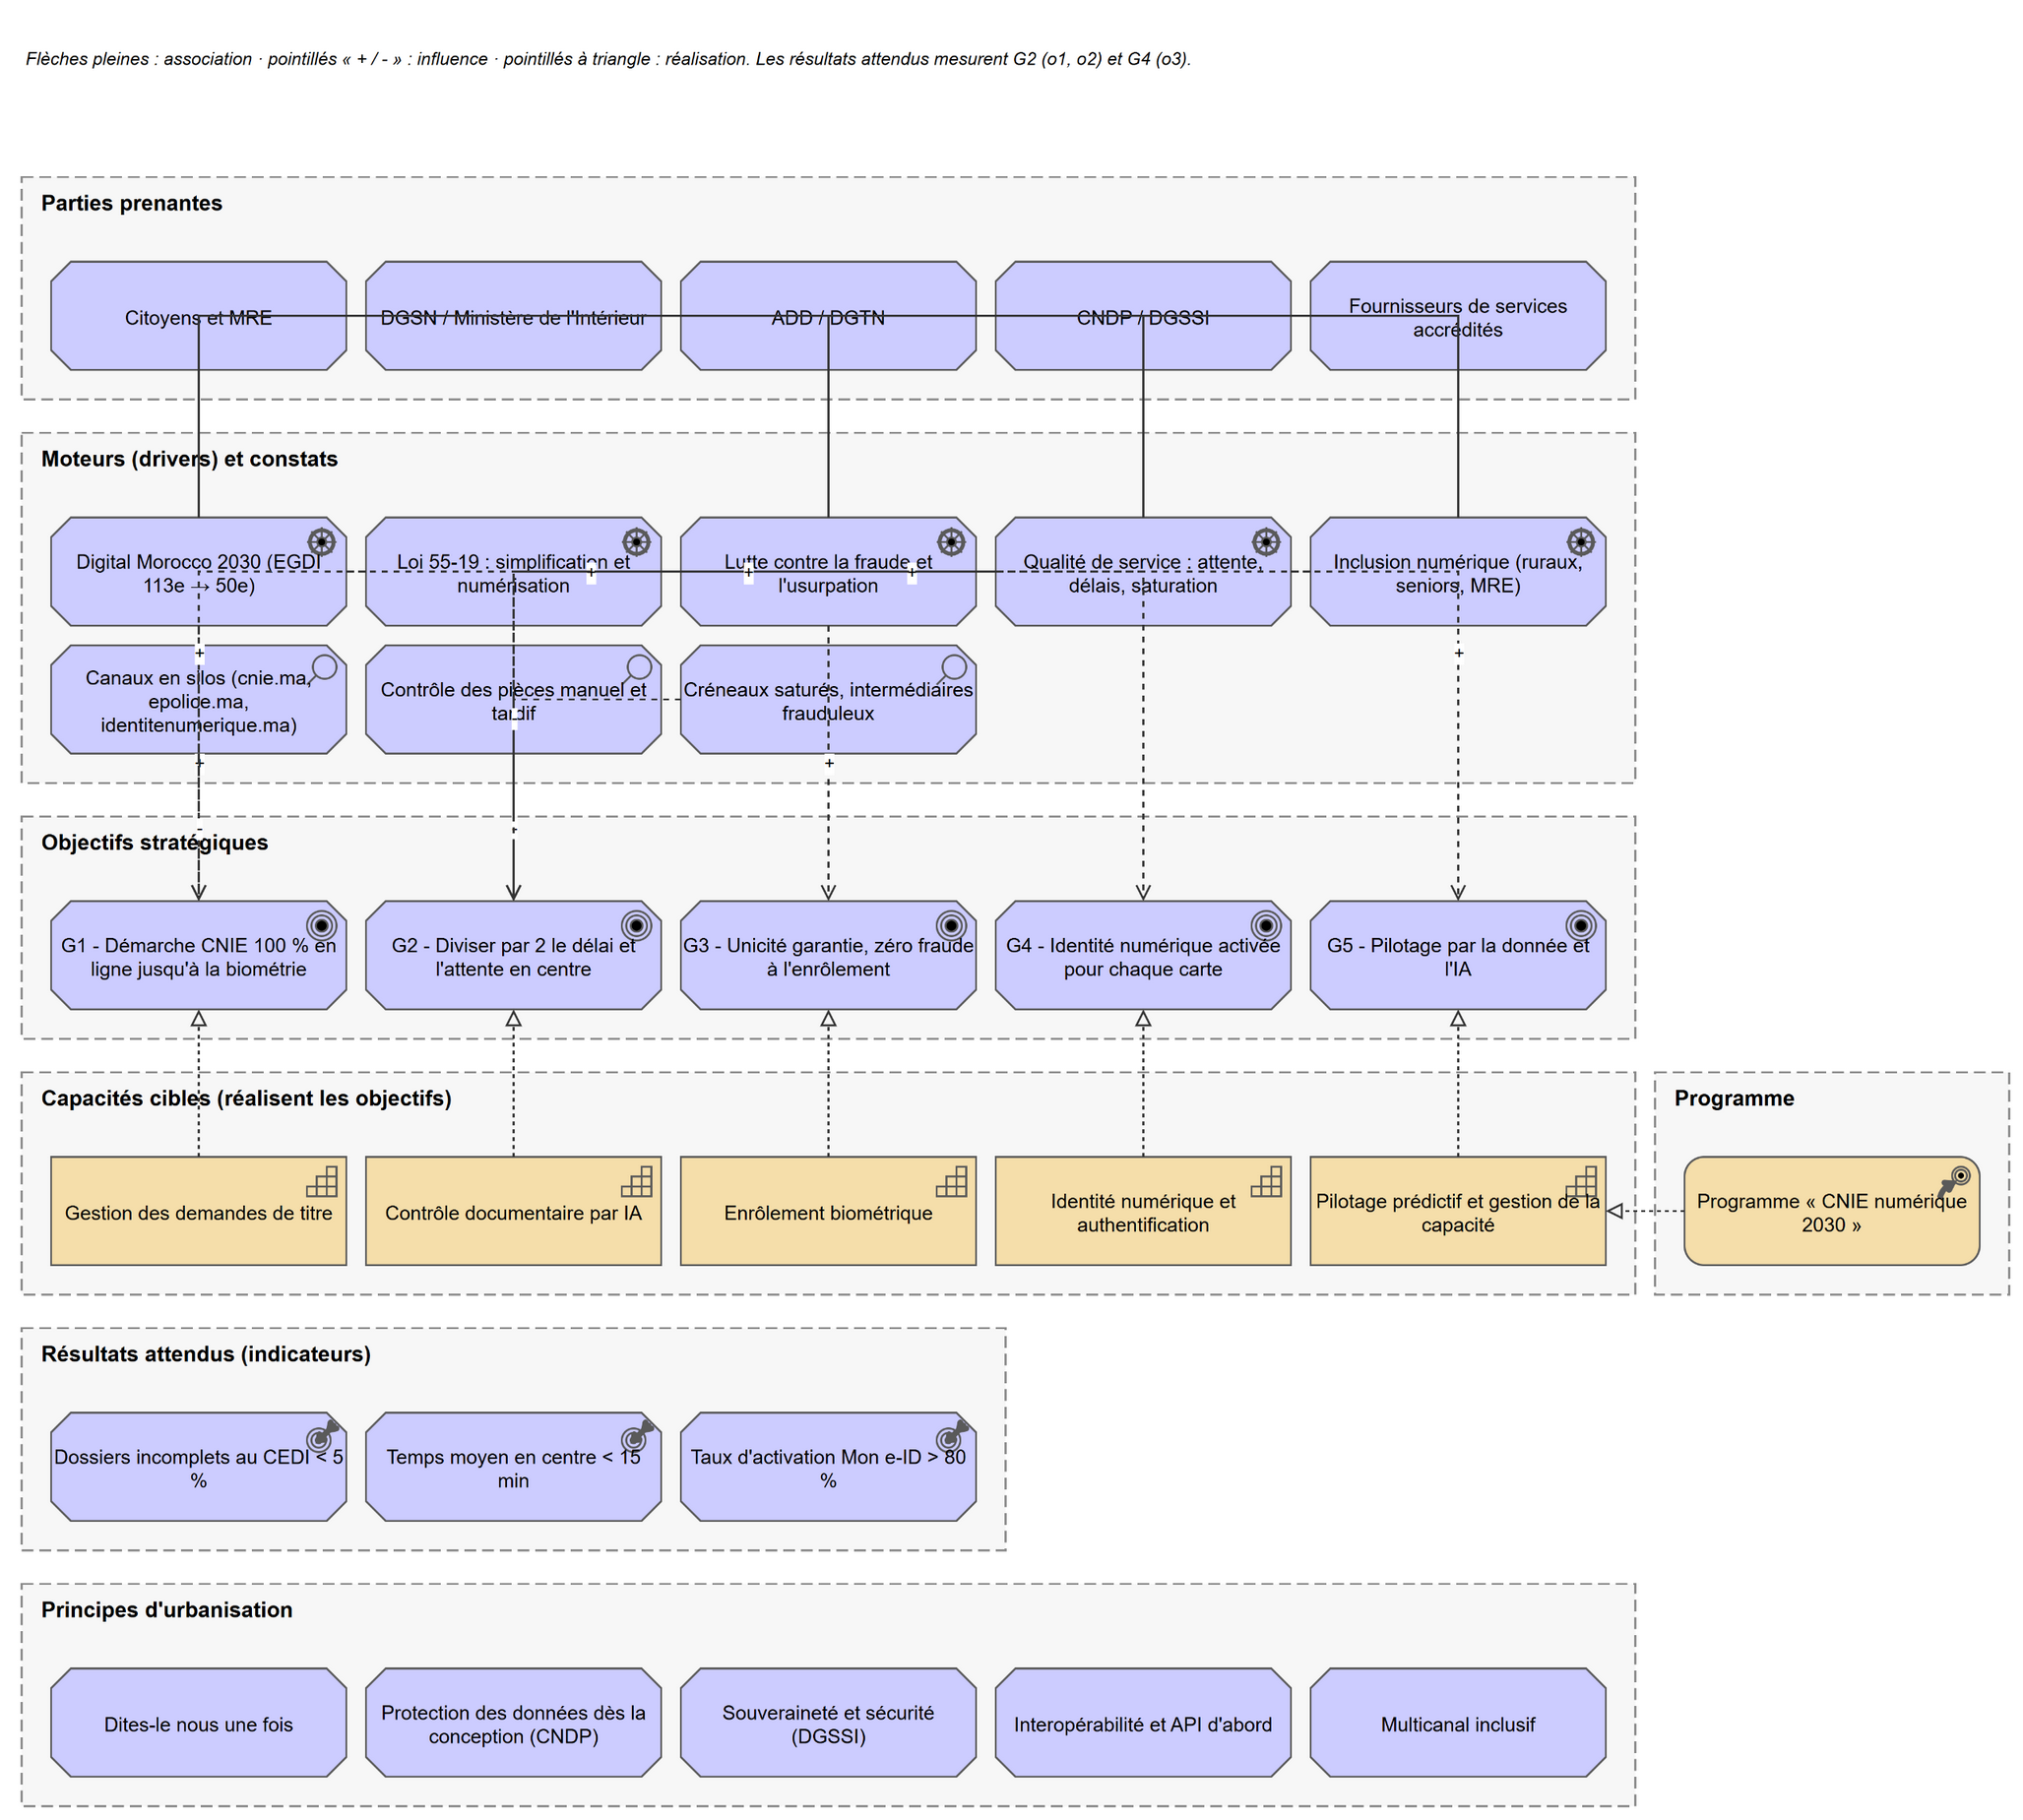
\includegraphics[width=0.95\textwidth]{archimate/V1_motivation.png}
\caption{Vue de motivation et de stratégie~: parties prenantes, moteurs, objectifs, principes et capacités cibles (ArchiMate).}
\label{fig:motivation}
\end{figure*}

\subsection{Principes d'urbanisation}
Cinq principes guident toutes les décisions d'architecture du présent rapport~:
\begin{enumerate}
  \item \textbf{Dites-le nous une fois}~: toute donnée connue de l'État (état civil, adresse, biométrie de référence) est réutilisée après consentement plutôt que redemandée.
  \item \textbf{Protection des données dès la conception}~: minimisation, consentement explicite, séparation des données d'usage et d'identification conformément aux recommandations de la CNDP \cite{cndp_0908}, et maintien du modèle «~les données sont sur la carte~» de la plateforme Tiers de Confiance.
  \item \textbf{Souveraineté et sécurité}~: hébergement national, cryptographie sous HSM, conformité DGSSI, aucune dépendance à un service d'IA hébergé hors du territoire pour les données biométriques.
  \item \textbf{Interopérabilité et API d'abord}~: chaque capacité est exposée par une interface documentée derrière une passerelle unique, ce qui permet d'intégrer les partenaires et de remplacer un composant sans toucher aux autres.
  \item \textbf{Multicanal inclusif}~: le canal numérique devient le canal principal, mais le guichet, l'assistance à domicile et l'assistant conversationnel en arabe, en français et en amazighe garantissent l'accès de tous.
\end{enumerate}

\subsection{Cas d'usage d'intelligence artificielle retenus}
L'intégration de l'IA n'est pas une fin en soi~: chaque cas d'usage répond à un objectif et s'insère à un point précis du processus (tableau~\ref{tab:ia}). Les modèles traitant des données biométriques sont soumis à une évaluation des biais démographiques avant mise en service, les écarts de performance entre groupes de population étant documentés dans la littérature \cite{grother2019frvt}.

\begin{table}[h]
\caption{Cas d'usage d'IA et ancrage dans le processus}
\label{tab:ia}
\centering
\small
\begin{tabularx}{\columnwidth}{lXl}
\toprule
\textbf{Code} & \textbf{Cas d'usage (technique)} & \textbf{Objectif} \\
\midrule
IA-1 & Assistant conversationnel multilingue guidant la saisie (modèle de langue avec recherche documentaire sur la base de connaissances DGSN) & G1, G2 \\
IA-2 & Contrôle documentaire automatique des pièces téléversées~: reconnaissance de caractères, cohérence avec la saisie, conformité de la photo aux critères ICAO \cite{icao9303} & G2 \\
IA-3 & Vérification biométrique à l'enrôlement~: dédoublonnage facial, détection du vivant, rapprochement avec la biométrie de référence & G3 \\
IA-4 & Prévision d'affluence par centre et recommandation de créneaux & G2, G5 \\
IA-5 & Détection d'anomalies sur les demandes et pilotage prédictif des délais & G3, G5 \\
\bottomrule
\end{tabularx}
\end{table}

\subsection{Capacités cibles}
Les objectifs sont réalisés par cinq capacités métier portées par le programme «~CNIE numérique 2030~»~: gestion des demandes de titre, enrôlement biométrique, identité numérique et authentification, contrôle documentaire par IA, pilotage prédictif et gestion de la capacité. Ces capacités constituent la charnière entre la stratégie et les cartographies qui suivent~: chaque bloc fonctionnel et chaque application de la cible contribue à au moins l'une d'elles.

\section{Cartographie métier cible}
\label{sec:metier}

\subsection{Services, acteurs et processus}
La vue métier (figure~\ref{fig:metier}) organise le périmètre autour de cinq services rendus~: la demande et le renouvellement de la CNIE, la prise de rendez-vous, le suivi, l'identité numérique et l'authentification offerte aux fournisseurs accrédités. Le processus principal P0 se décompose en quatre sous-processus enchaînés~: SP1 pré-demande, contrôle des pièces et rendez-vous (nouveau)~; SP2 enrôlement au CEDI (à faire évoluer)~; SP3 production et personnalisation (conservé)~; SP4 notification, remise et activation de l'identité numérique (à faire évoluer). Un nouvel acteur apparaît~: l'\emph{agent instructeur}, qui traite à distance les dossiers que le contrôle automatique n'a pas pu trancher, ce qui déplace une partie de la charge des guichets vers un back-office mutualisé.

\begin{figure}[h]
\centering
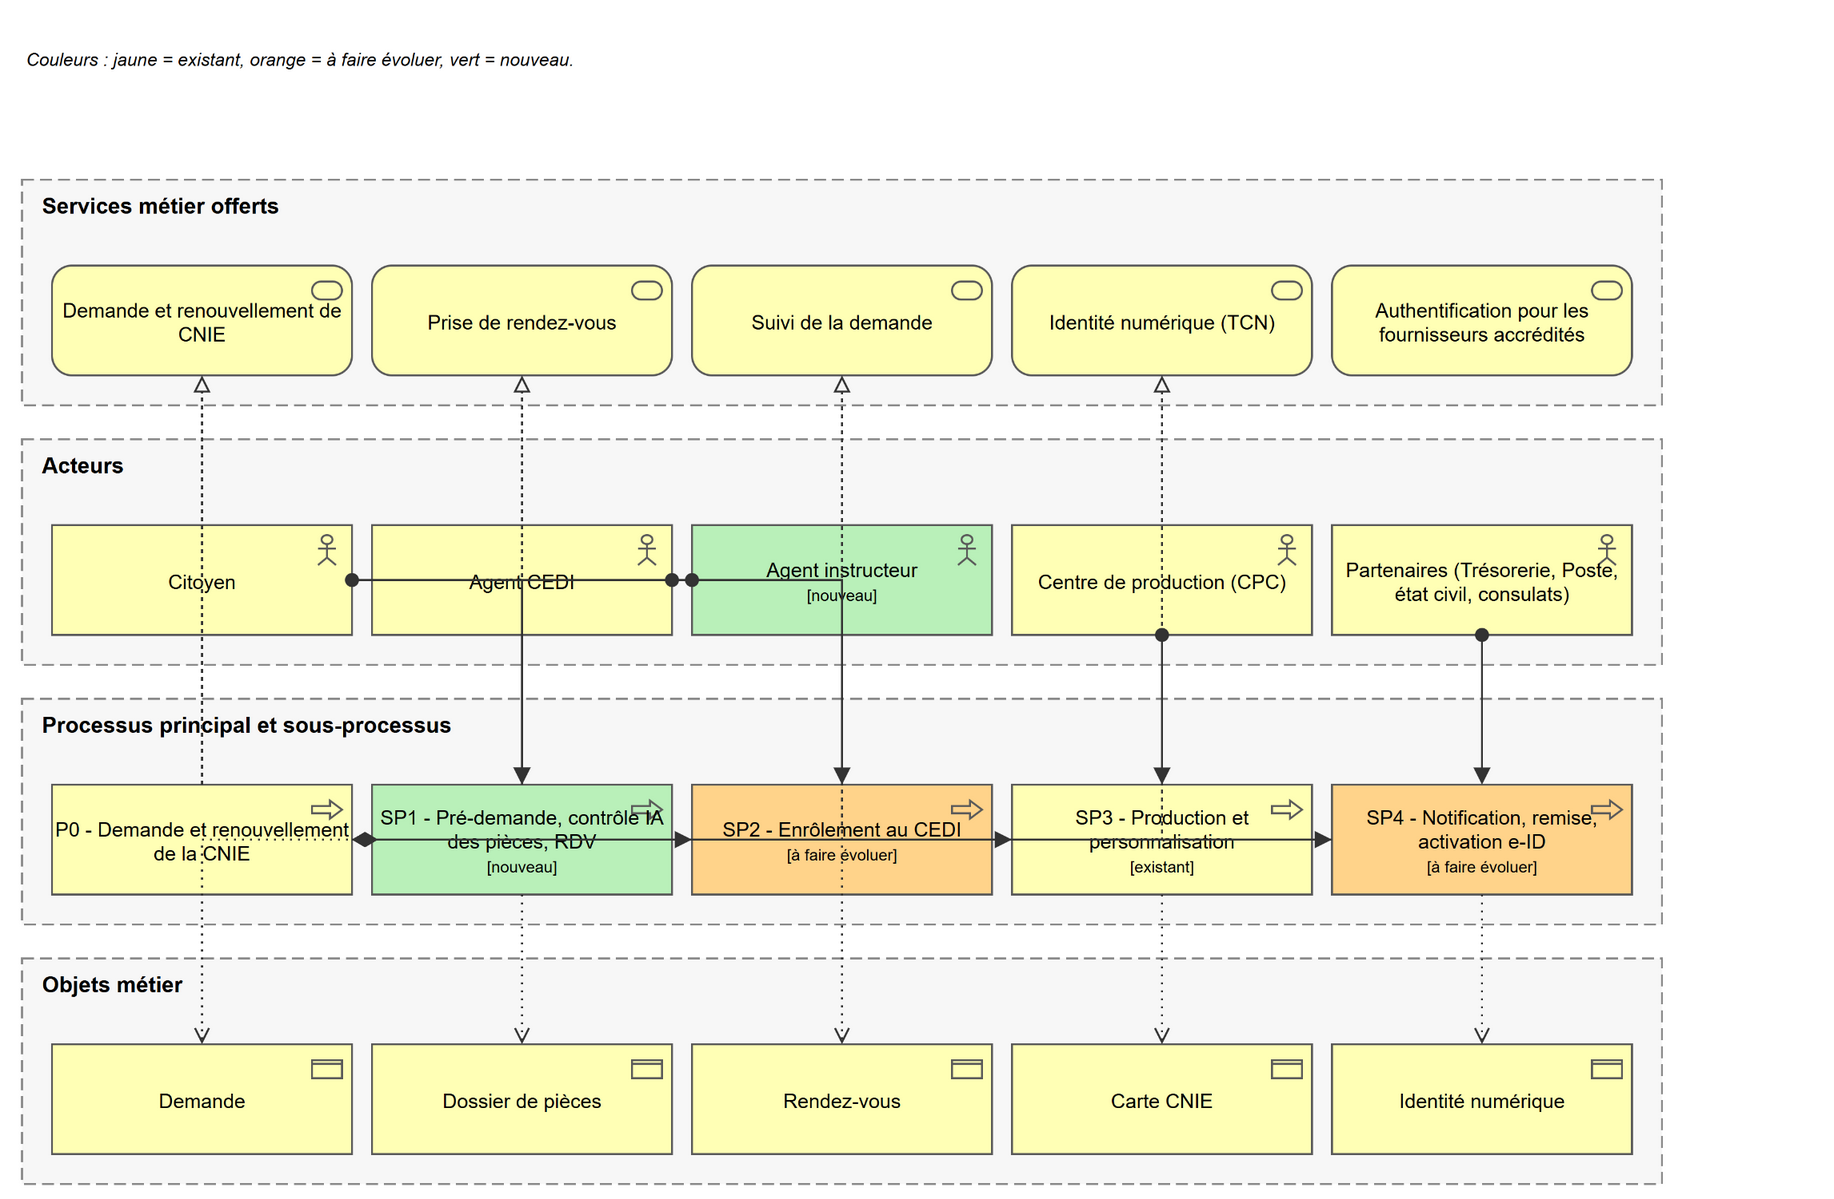
\includegraphics[width=\columnwidth]{archimate/V2_metier.png}
\caption{Vue métier cible~: services, acteurs, processus et objets métier.}
\label{fig:metier}
\end{figure}

\subsection{Le processus cible}
La figure~\ref{fig:bpmn-tobe} présente le processus P0 cible modélisé sous Blueworks Live. Par rapport à l'existant, six transformations sont introduites~:
\begin{enumerate}
  \item \textbf{Entrée par l'identité numérique}~: le citoyen déjà porteur d'une carte s'authentifie via la plateforme Tiers de Confiance et sa demande est pré-remplie à partir de la carte et de l'état civil (principe «~dites-le nous une fois~»).
  \item \textbf{Contrôle documentaire immédiat (IA-2)}~: les pièces téléversées sont analysées en quelques secondes~; un score de conformité oriente la demande vers la confirmation, vers une correction par le citoyen ou vers l'instruction humaine. Le dossier incomplet est détecté avant le déplacement, et non après.
  \item \textbf{Paiement intégré}~: l'e-timbre est vérifié en ligne au moment de la demande, sans ressaisie de code.
  \item \textbf{Créneaux recommandés (IA-4)}~: la prévision d'affluence propose les créneaux les moins chargés, avec convocation par QR code et rappels automatiques.
  \item \textbf{Enrôlement allégé et sécurisé (IA-3)}~: au CEDI, l'agent scanne la convocation et ne réalise que la capture biométrique~; la vérification d'unicité et la détection de fraude sont exécutées en temps réel et toute alerte est routée vers l'instructeur.
  \item \textbf{Remise au choix et activation}~: la carte est retirée au centre ou livrée à domicile avec authentification du porteur, puis la carte numérique est activée dans l'application «~Mon e-ID~», ce qui clôt le processus sur un citoyen immédiatement équipé pour les services en ligne.
\end{enumerate}

\begin{sidewaysfigure*}
\centering
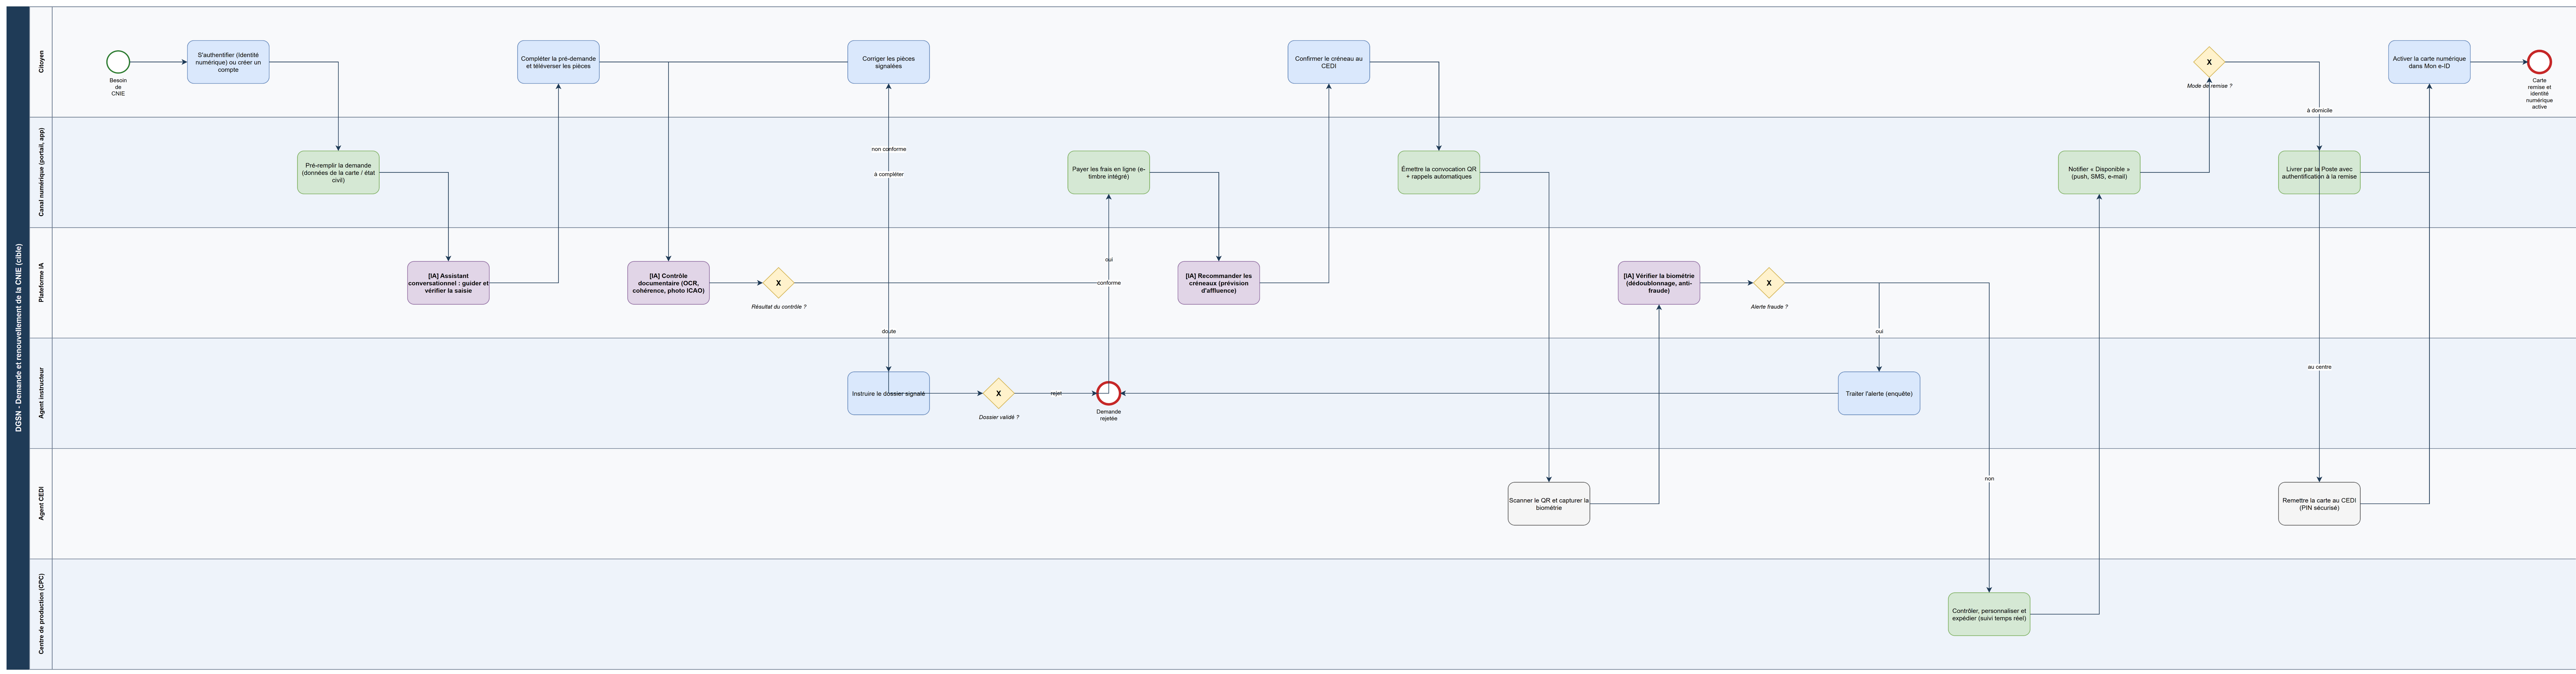
\includegraphics[width=\textwidth]{bpmn/P0_demande_cnie_tobe.png}
\caption{Processus P0 cible (to-be)~: les tâches en violet sont réalisées par la plateforme d'IA~; deux nouveaux couloirs apparaissent (plateforme IA, agent instructeur).}
\label{fig:bpmn-tobe}
\end{sidewaysfigure*}

\subsection{Indicateurs de performance du processus}
Pour piloter la transformation, nous proposons de suivre~: le taux de dossiers conformes au premier contrôle, le taux de dossiers incomplets constatés au guichet (cible $<$~5~\%), le délai médian entre la demande et la remise, le temps moyen de passage en centre, le taux d'occupation des créneaux par centre, le nombre d'alertes de fraude confirmées, et le taux d'activation de l'identité numérique à la remise. Ces indicateurs alimentent la zone de pilotage décrite dans la cartographie fonctionnelle.

\section{Cartographie fonctionnelle cible}
\label{sec:fonctionnel}

\subsection{Plan d'occupation des sols}
La cartographie fonctionnelle (figure~\ref{fig:fonctionnel}) décrit ce que le système cible doit savoir faire, indépendamment des logiciels qui le feront. Elle est organisée en six zones, conformément aux pratiques d'urbanisation \cite{longepe2009}~: une zone d'\emph{échange} regroupant les canaux, une zone \emph{opérationnelle} portant le cœur du métier, une zone de \emph{support}, une zone de \emph{pilotage et d'IA}, une zone de \emph{ressources} et une zone de \emph{référentiels et d'échanges} avec les systèmes externes. Chaque bloc porte son statut~: \tagE~existant, \tagV~à faire évoluer, \tagN~nouveau.

\begin{figure*}[t]
\centering
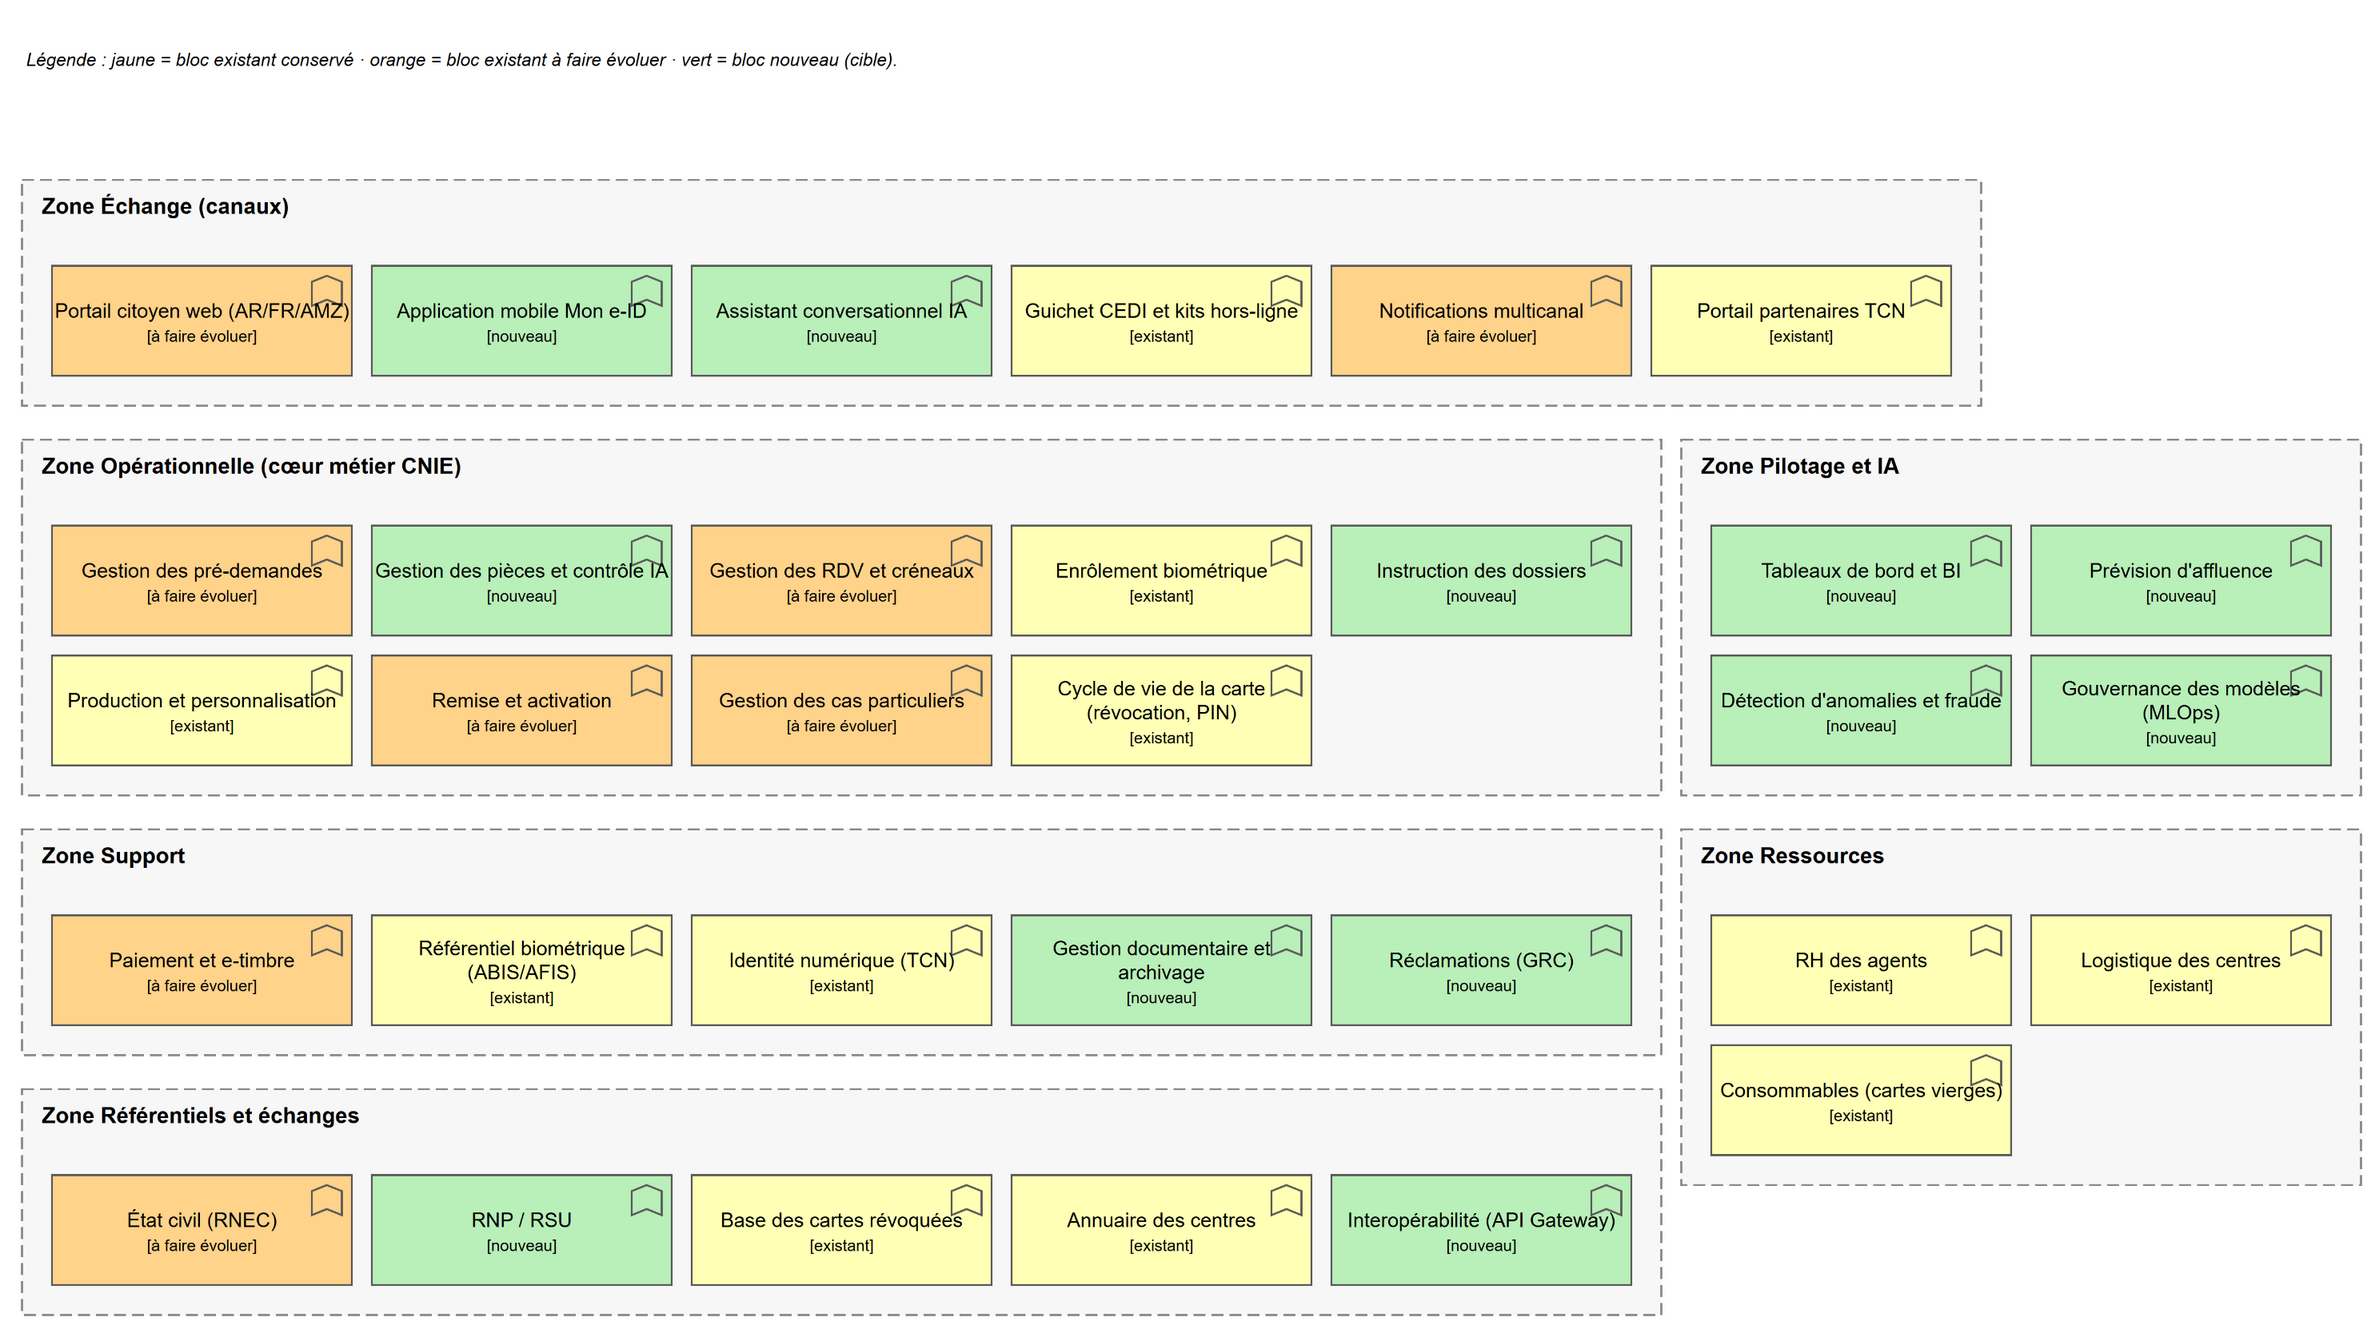
\includegraphics[width=0.98\textwidth]{archimate/V3_fonctionnel.png}
\caption{Plan d'occupation des sols fonctionnel cible~: 32 blocs répartis en six zones, avec mise en évidence des blocs existants, à faire évoluer et nouveaux.}
\label{fig:fonctionnel}
\end{figure*}

\subsection{Lecture zone par zone}
\paragraph{Zone Échange} Le portail web est conservé mais refondu (multilingue, accessible, adaptatif), tandis que deux canaux nouveaux apparaissent~: l'application mobile «~Mon e-ID~», qui fusionne la carte numérique et le suivi des demandes, et l'assistant conversationnel (IA-1). Le guichet des CEDI et les kits hors-ligne de la plateforme Tiers de Confiance restent indispensables pour l'inclusion. Les notifications deviennent multicanal (SMS, e-mail, notification mobile).

\paragraph{Zone Opérationnelle} Deux blocs nouveaux concentrent la valeur de la cible~: la \emph{gestion des pièces et contrôle IA} (IA-2) et l'\emph{instruction des dossiers}, qui outille le nouvel acteur back-office. La gestion des pré-demandes, des rendez-vous, de la remise et des cas particuliers évolue pour s'intégrer au moteur de processus. L'enrôlement biométrique, la production et le cycle de vie de la carte sont conservés tels quels, car ils reposent sur des équipements et des procédures de sécurité éprouvés.

\paragraph{Zone Support} Le paiement évolue vers une vérification en ligne de l'e-timbre. Le référentiel biométrique et l'identité numérique existent déjà. Deux fonctions nouvelles s'ajoutent~: la gestion documentaire avec archivage à valeur probante, rendue nécessaire par la dématérialisation des pièces, et la gestion des réclamations.

\paragraph{Zone Pilotage et IA} Entièrement nouvelle, elle regroupe les tableaux de bord, la prévision d'affluence (IA-4), la détection d'anomalies et de fraude (IA-5) et la gouvernance des modèles (suivi des performances, des biais et des versions), sans laquelle l'usage de l'IA dans un service régalien ne serait pas acceptable.

\paragraph{Zones Ressources et Référentiels} Les ressources humaines, logistiques et les consommables sont hors du périmètre de transformation. En revanche, la zone des référentiels s'ouvre~: l'accès à l'état civil devient automatisé, l'interconnexion au Registre National de la Population est préparée, et une fonction d'interopérabilité unique (passerelle d'API) encadre tous les échanges.

\subsection{Matrice de couverture}
Le tableau~\ref{tab:couverture} vérifie que chaque capacité stratégique est portée par au moins un bloc fonctionnel, et que chaque bloc nouveau se justifie par un objectif.

\begin{table}[h]
\caption{Couverture des capacités cibles par les blocs fonctionnels}
\label{tab:couverture}
\centering
\small
\begin{tabularx}{\columnwidth}{lX}
\toprule
\textbf{Capacité} & \textbf{Blocs fonctionnels contributeurs} \\
\midrule
Gestion des demandes de titre & Pré-demandes \tagV, pièces et contrôle IA \tagN, RDV \tagV, instruction \tagN, remise \tagV, cas particuliers \tagV \\
Enrôlement biométrique & Enrôlement \tagE, référentiel biométrique \tagE, guichet et kits \tagE \\
Identité numérique et authentification & Identité numérique TCN \tagE, app Mon e-ID \tagN, portail partenaires \tagE \\
Contrôle documentaire par IA & Pièces et contrôle IA \tagN, gestion documentaire \tagN, assistant \tagN \\
Pilotage prédictif & BI \tagN, prévision \tagN, anomalies \tagN, MLOps \tagN \\
\bottomrule
\end{tabularx}
\end{table}

\section{Cartographie applicative cible et prototype}
\label{sec:applicatif}

\subsection{Composants applicatifs}
La cartographie applicative (figure~\ref{fig:applicatif}) traduit les blocs fonctionnels en quinze composants logiciels, regroupés en sept quartiers~: canaux, identité numérique, orchestration et services d'IA, cœur métier, support et données, intégration, et systèmes externes. Le choix structurant est l'introduction d'un \textbf{moteur de processus} (APP-04) qui orchestre la demande de bout en bout et porte les règles de routage~; les canaux ne contiennent plus de logique métier et les services d'IA sont des composants autonomes, appelés par le moteur, remplaçables indépendamment. Une \textbf{passerelle d'API} (APP-11) centralise les échanges avec l'état civil, la Trésorerie, Barid Al-Maghrib et les consulats, ce qui supprime les interfaces point à point.

\begin{figure*}[t]
\centering
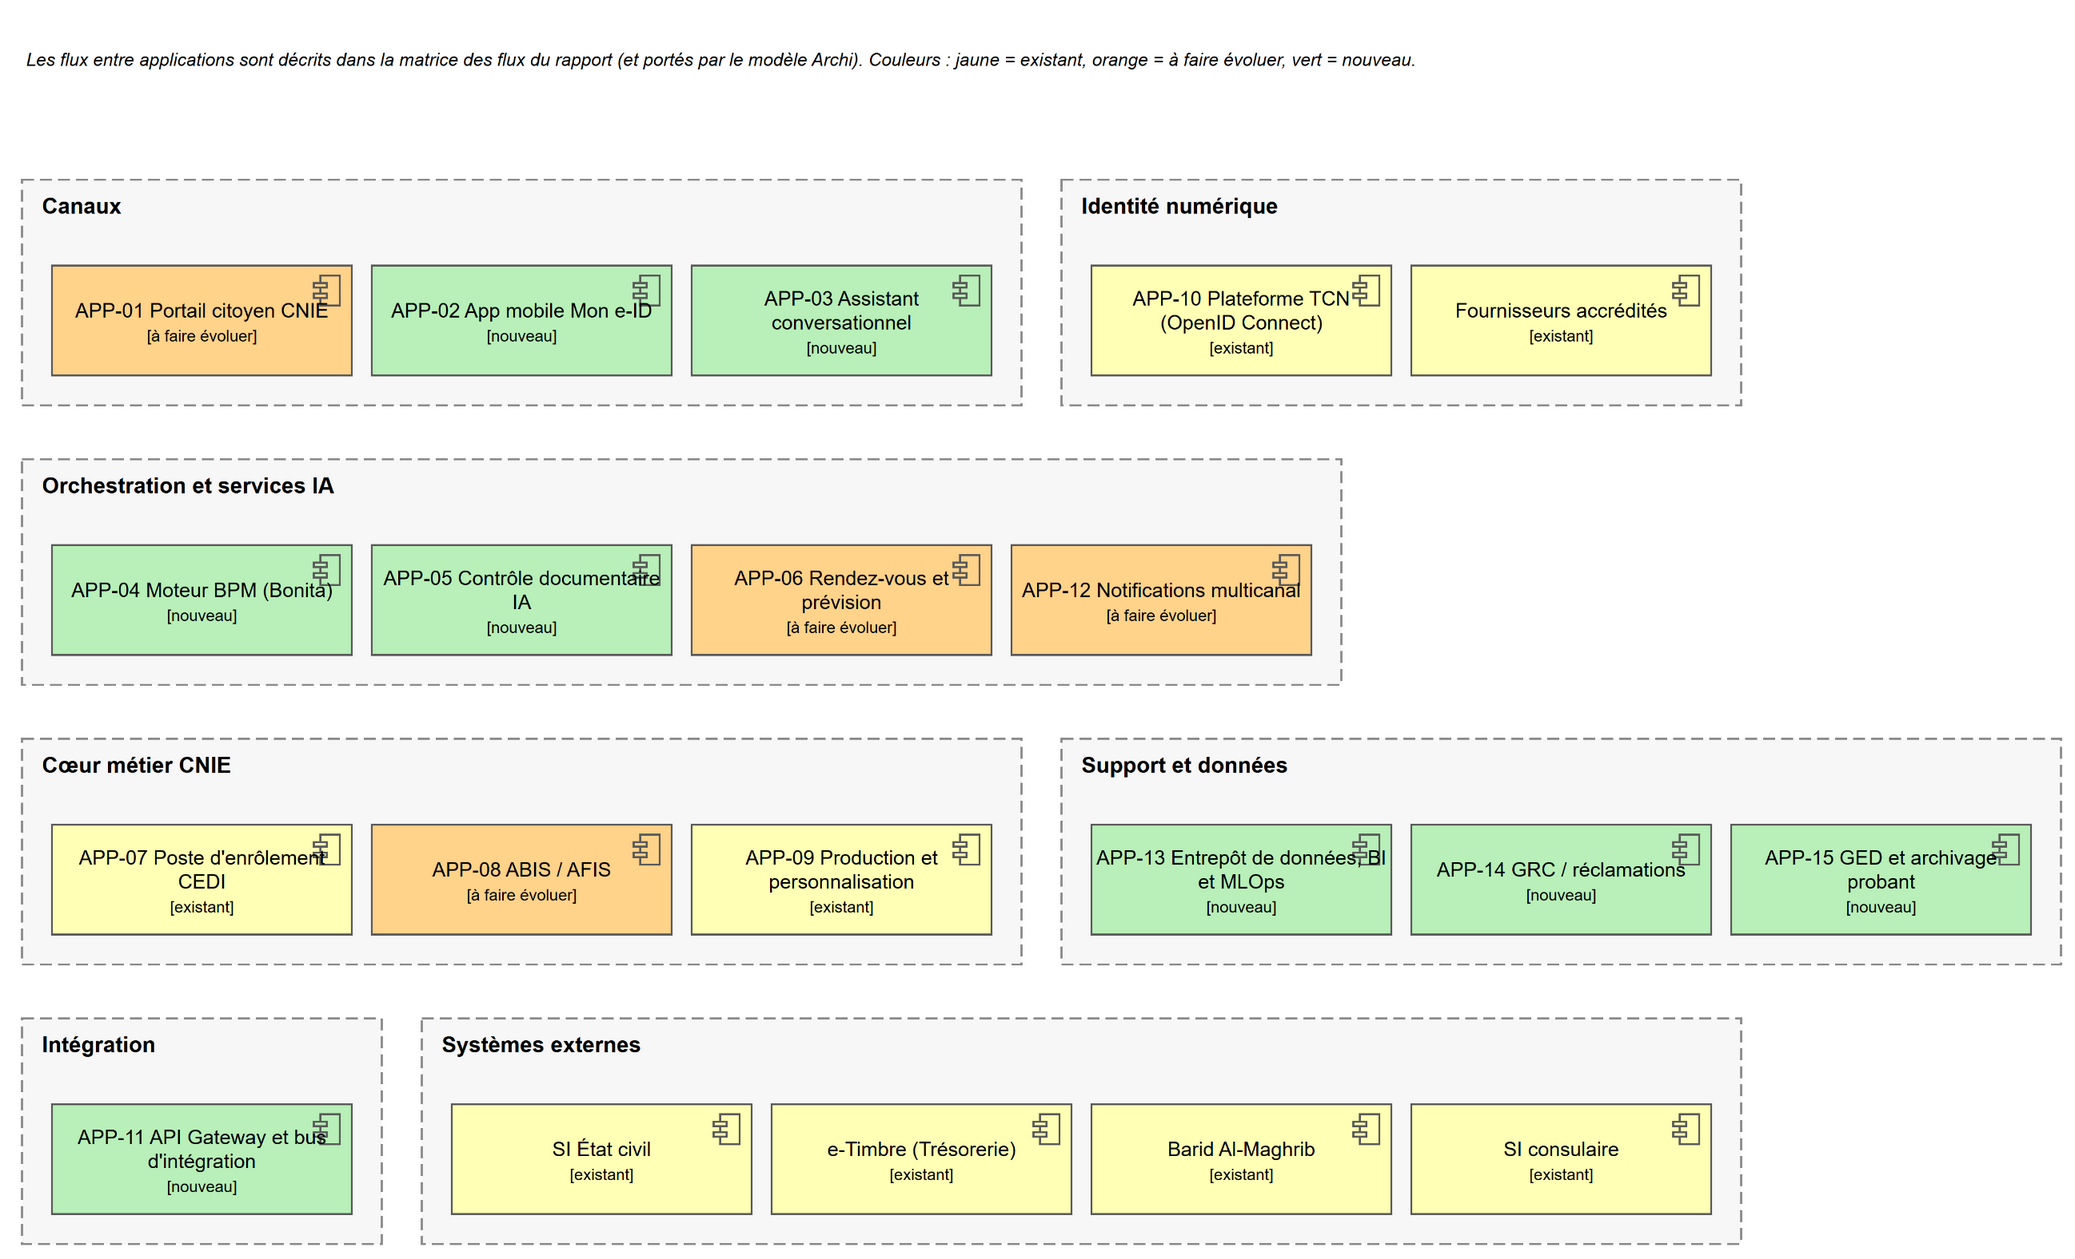
\includegraphics[width=0.98\textwidth]{archimate/V4_applicatif.png}
\caption{Cartographie applicative cible~: quinze composants et cinq systèmes externes, avec leur statut.}
\label{fig:applicatif}
\end{figure*}

\subsection{Matrice des flux}
Le tableau~\ref{tab:flux} décrit les principaux flux entre composants. Tous transitent par le bus d'événements de la zone applicative (publication d'événements de statut) ou par des appels d'API synchrones sécurisés par jetons~; aucune base de données n'est partagée entre deux composants.

\begin{table}[h]
\caption{Principaux flux applicatifs cibles}
\label{tab:flux}
\centering
\small
\begin{tabularx}{\columnwidth}{llX}
\toprule
\textbf{Source} & \textbf{Cible} & \textbf{Contenu du flux} \\
\midrule
APP-01 / 02 & APP-04 & Création et mise à jour de la demande, pièces téléversées \\
APP-10 & APP-01 / 02 & Authentification du citoyen (OpenID Connect), attributs d'identité après consentement \\
APP-03 & APP-01 / 02 & Réponses de l'assistant, aide contextuelle à la saisie \\
APP-04 & APP-05 & Pièces à contrôler~; retour du score de conformité et des anomalies \\
APP-04 & APP-06 & Demande de créneaux~; retour des créneaux recommandés \\
APP-04 & APP-11 & Vérification de l'e-timbre, récupération de l'acte d'état civil, ordre de livraison \\
APP-04 & APP-07 & Convocation (QR code) et dossier pré-qualifié \\
APP-07 & APP-08 & Gabarits biométriques pour dédoublonnage et contrôle de fraude \\
APP-08 & APP-09 & Dossier validé pour production \\
APP-09 & APP-04 & Événements de statut (en production, disponible, expédiée) \\
APP-04 & APP-12 & Événements à notifier (SMS, e-mail, notification mobile) \\
APP-04 / 06 / 09 & APP-13 & Journal d'événements anonymisé pour la BI et l'entraînement des modèles \\
APP-04 / 09 & APP-15 & Pièces et récépissés à archiver avec horodatage \\
APP-14 & APP-04 & Réclamations rattachées à une demande \\
Fournisseurs & APP-10 & Délégation d'authentification (inchangée) \\
\bottomrule
\end{tabularx}
\end{table}

\subsection{Plateforme d'IA}
Les composants APP-03, APP-05, APP-06 et APP-08 consomment une plateforme d'inférence commune (zone IA de l'architecture technique). Trois choix de conception protègent la DGSN~: les modèles sont hébergés sur site, les données biométriques ne quittent jamais la zone sécurisée, et chaque modèle est versionné dans un registre avec ses métriques de performance et d'équité, suivies par le composant MLOps d'APP-13. L'assistant conversationnel n'accède qu'à une base de connaissances documentaire validée et ne traite aucune donnée d'identité.

\subsection{Prototype Bonita du sous-processus SP1}
Le sous-processus SP1 a été implémenté sous Bonita Studio Community afin de valider l'orchestration, les règles de décision et les interfaces (figure~\ref{fig:bonita-proc}). Le modèle de données métier comprend quatre objets~: \texttt{DemandeCNIE} (identité, état civil, adresse, contact, statut, score), \texttt{PieceJustificative} (type, fichier, verdict de l'IA), \texttt{RendezVous} (centre, date, créneau, QR code) et \texttt{Centre} (capacité et charge prévue). Trois acteurs sont définis~: le citoyen, initiateur du processus~; l'agent instructeur~; et les tâches de service automatiques.

\begin{figure}[h]
\centering
\IfFileExists{figures/bonita/bonita-diagramme.png}{\includegraphics[width=\columnwidth]{bonita/bonita-diagramme.png}}{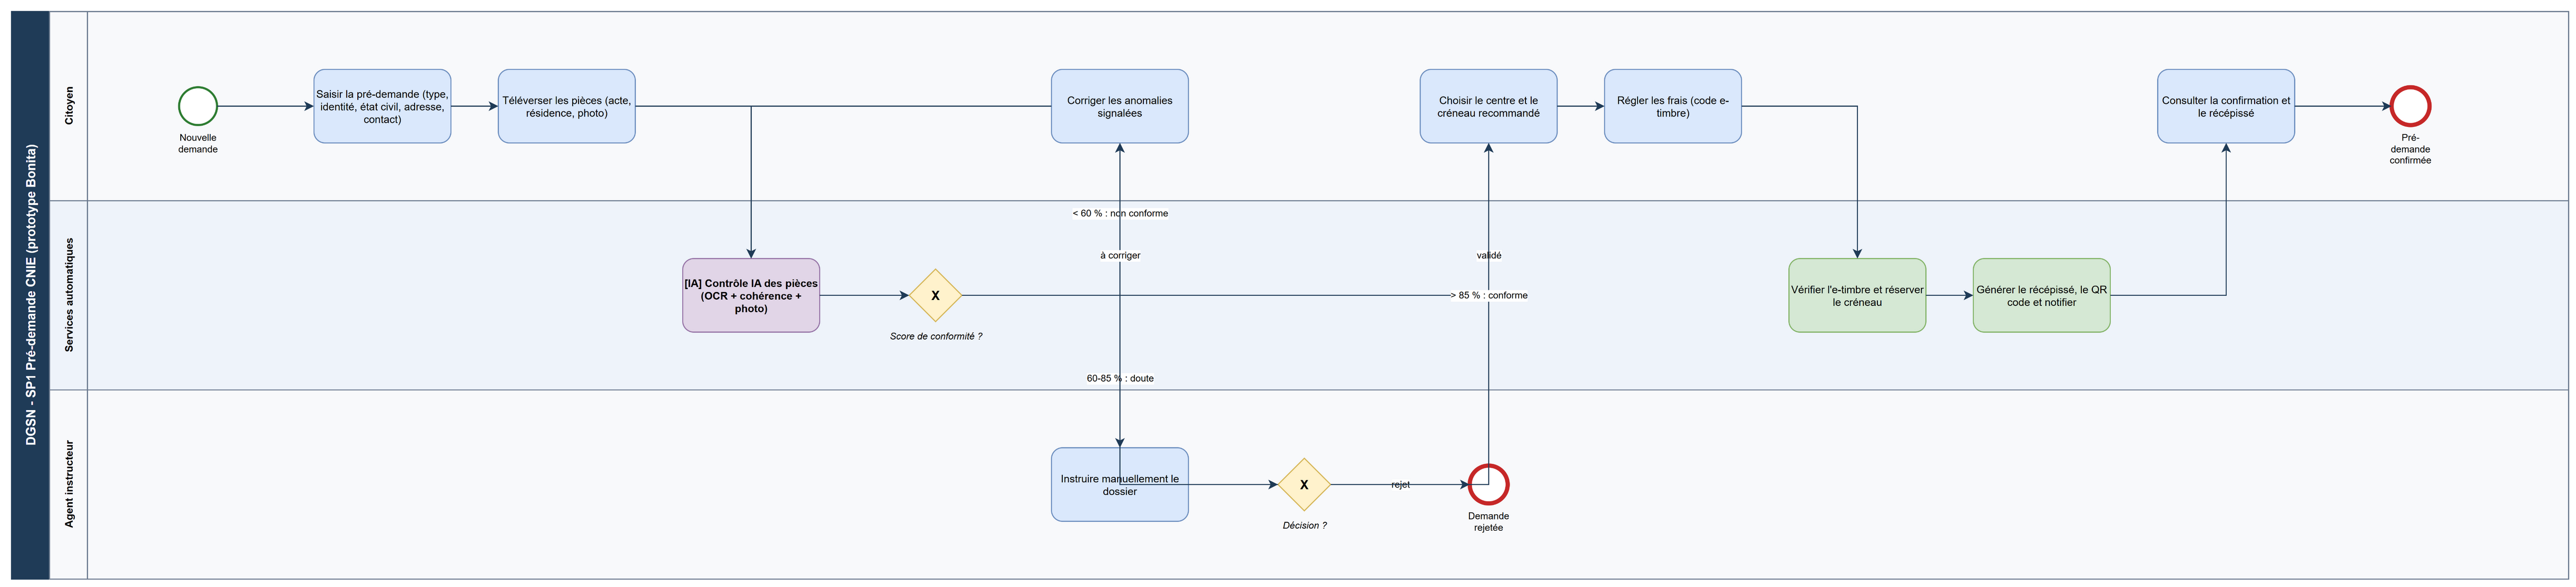
\includegraphics[width=\columnwidth]{bpmn/SP1_predemande_bonita.png}}
\caption{Sous-processus SP1 implémenté sous Bonita~: pré-demande, contrôle des pièces, instruction, rendez-vous et paiement.}
\label{fig:bonita-proc}
\end{figure}

Le parcours comporte six écrans (figure~\ref{fig:bonita-ecrans})~: (1)~saisie de la pré-demande avec validation des formats~; (2)~téléversement des pièces~; (3)~résultat du contrôle automatique sous forme de jauge de conformité et de liste d'anomalies, avec reprise des seules pièces à corriger~; (4)~choix du centre, affichage de sa charge prévue et des créneaux recommandés~; (5)~saisie du code e-timbre~; (6)~confirmation avec numéro de demande et QR code de convocation. Un septième écran, réservé à l'agent instructeur, présente le dossier et les anomalies et recueille sa décision.

Le service de contrôle documentaire est simulé par un connecteur de script qui calcule un score à partir de la présence des pièces et de règles de nommage~; la passerelle exclusive route la demande selon trois seuils (conforme au-delà de 85, instruction humaine entre 60 et 85, correction en deçà). Cette simulation suffit à démontrer la logique du processus~; en production, le connecteur appelle l'API du composant APP-05.

\begin{figure*}[t]
\centering
\IfFileExists{figures/bonita/F1-predemande.png}{%
\begin{subfigure}[t]{0.32\textwidth}\includegraphics[width=\textwidth]{bonita/F1-predemande.png}\caption{Pré-demande}\end{subfigure}\hfill
\begin{subfigure}[t]{0.32\textwidth}\includegraphics[width=\textwidth]{bonita/F3-resultat-ia.png}\caption{Résultat du contrôle IA}\end{subfigure}\hfill
\begin{subfigure}[t]{0.32\textwidth}\includegraphics[width=\textwidth]{bonita/F4-creneau.png}\caption{Créneaux recommandés}\end{subfigure}}{%
\fbox{\parbox{0.9\textwidth}{\centering\vspace{2cm}Captures d'écran des formulaires Bonita (à insérer~: \texttt{figures/bonita/F1-predemande.png}, \texttt{F3-resultat-ia.png}, \texttt{F4-creneau.png})\vspace{2cm}}}}
\caption{Interfaces du prototype Bonita (UI Designer).}
\label{fig:bonita-ecrans}
\end{figure*}

\section{Architecture technique cible}
\label{sec:technique}

\subsection{Principes techniques}
L'architecture technique (figure~\ref{fig:technique}) découle des principes de souveraineté, de sécurité et d'interopérabilité. Elle repose sur un hébergement dans un cloud souverain conforme aux exigences de la DGSSI, sur une segmentation en zones étanches, sur des composants conteneurisés orchestrés par Kubernetes, et sur un bus d'événements qui découple les applications. Les sites physiques (CEDI, centres de production) restent connectés par le réseau interministériel sécurisé.

\begin{figure*}[t]
\centering
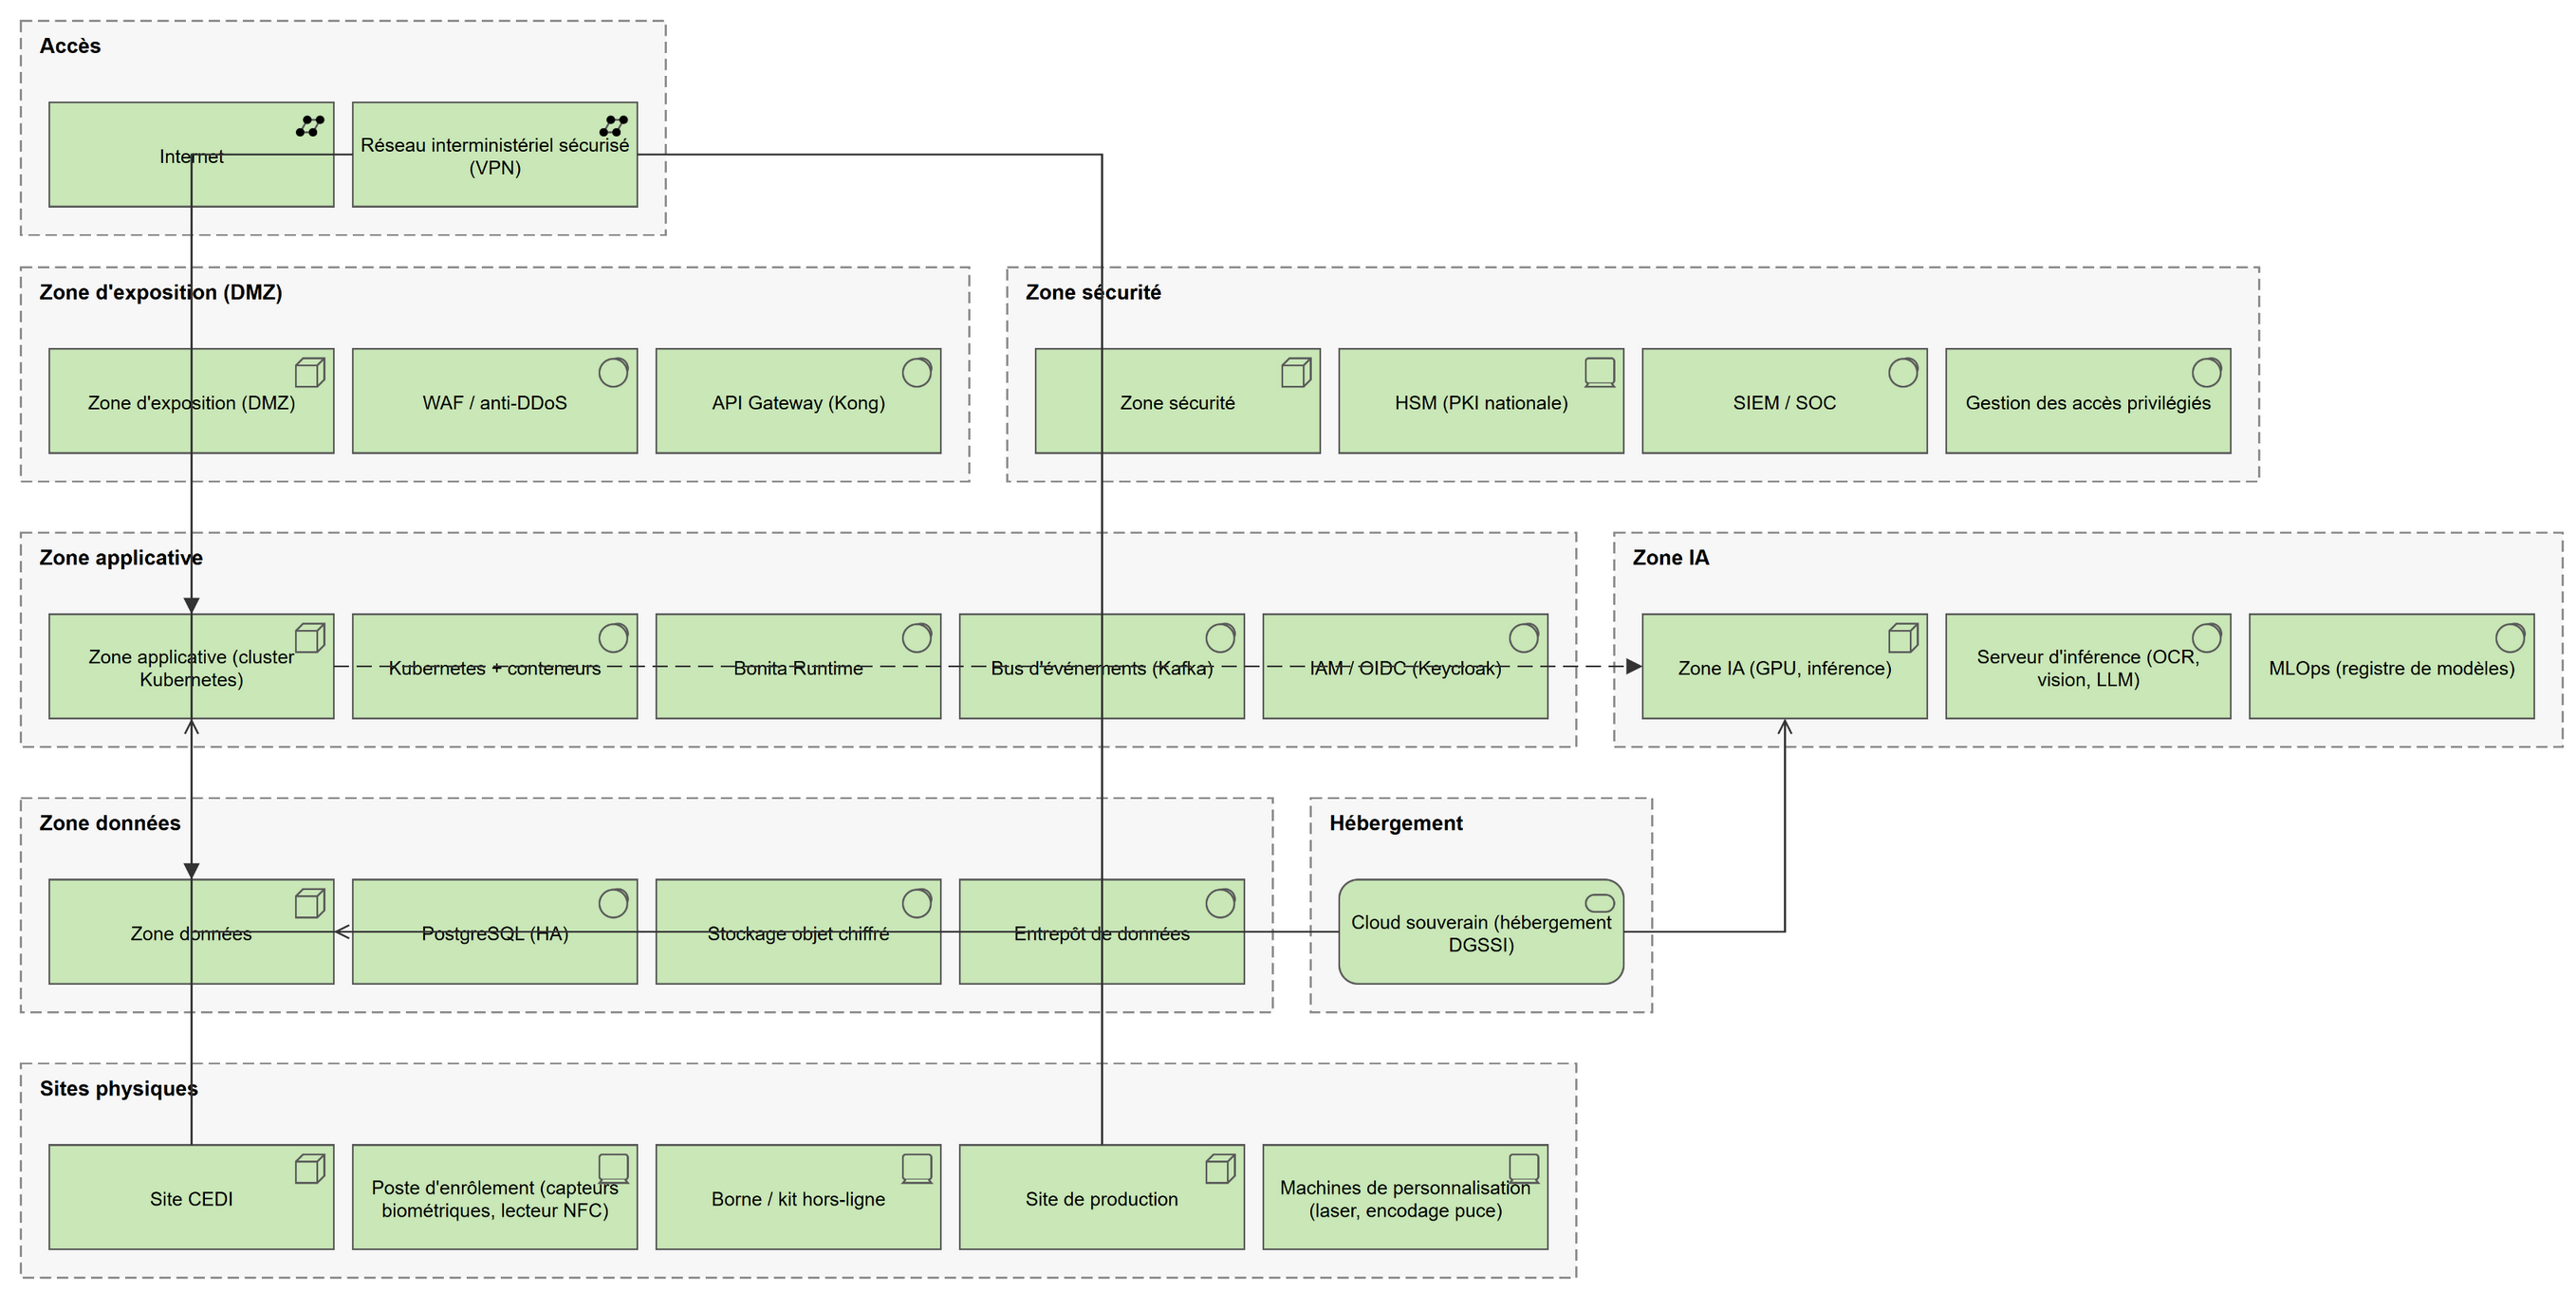
\includegraphics[width=0.98\textwidth]{archimate/V5_technique.png}
\caption{Architecture technique cible~: zones d'exposition, de sécurité, applicative, d'IA et de données~; sites physiques.}
\label{fig:technique}
\end{figure*}

\subsection{Zones}
\paragraph{Zone d'exposition} Un pare-feu applicatif et une protection contre le déni de service filtrent les accès depuis Internet. La passerelle d'API (APP-11) y est exposée~; elle applique l'authentification des clients, les quotas et la journalisation. Les canaux citoyens (portail, application mobile) ne dialoguent qu'avec cette passerelle.
\paragraph{Zone applicative} Le cluster Kubernetes héberge le moteur Bonita, les services métier et le bus d'événements. Le serveur d'identité (OpenID Connect) fédère les authentifications internes et délègue celles des citoyens à la plateforme Tiers de Confiance, qui reste un système distinct, conformément à son modèle sans registre central \cite{dgsn2023tcn}.
\paragraph{Zone de données} Les bases relationnelles en haute disponibilité portent les demandes et les rendez-vous~; un stockage objet chiffré conserve les pièces téléversées avec une durée de rétention limitée~; l'entrepôt de données alimente la BI à partir de données pseudonymisées.
\paragraph{Zone d'IA} Un serveur d'inférence dédié, doté d'accélérateurs graphiques, exécute les modèles de reconnaissance de caractères, de vision, de prévision et le modèle de langue de l'assistant. Le registre de modèles et la chaîne MLOps assurent le versionnement, les tests de non-régression et la surveillance de la dérive. Aucun flux de cette zone ne sort du territoire.
\paragraph{Zone de sécurité} Les modules matériels de sécurité (HSM) protègent les clés de la PKI nationale utilisées pour la personnalisation des puces et la signature des récépissés~; un SIEM centralise les journaux et alimente le centre opérationnel de sécurité~; la gestion des accès privilégiés encadre les administrateurs.
\paragraph{Sites physiques} Les postes d'enrôlement des CEDI (capteurs biométriques, lecteur NFC, scanner de QR code) et les kits hors-ligne fonctionnent en mode dégradé en cas de coupure réseau et se resynchronisent ensuite. Les centres de production conservent leurs machines de personnalisation, intégrées par le bus d'événements pour la remontée des statuts.

\subsection{Sécurité et conformité}
Le tableau~\ref{tab:secu} résume les mesures de sécurité associées aux principaux risques. Les niveaux d'assurance d'identité et d'authentification s'inspirent des catégories définies par les référentiels internationaux \cite{nist80063}~: l'accès à une demande en cours requiert une authentification forte via l'identité numérique, et la remise à domicile exige une vérification biométrique du porteur.

\begin{table}[h]
\caption{Risques et mesures de sécurité}
\label{tab:secu}
\centering
\small
\begin{tabularx}{\columnwidth}{lX}
\toprule
\textbf{Risque} & \textbf{Mesure} \\
\midrule
Usurpation d'identité en ligne & Authentification forte OpenID Connect via la plateforme Tiers de Confiance, détection du vivant à l'enrôlement \\
Fuite de pièces justificatives & Chiffrement au repos et en transit, rétention limitée, accès journalisés, séparation des zones \\
Fraude documentaire & Contrôle automatique des pièces, rapprochement avec l'état civil, instruction humaine des cas douteux \\
Compromission des clés & HSM certifiés, double contrôle des opérations, rotation des clés \\
Biais ou dérive des modèles & Évaluation d'équité avant mise en service, surveillance continue, décision humaine sur toute alerte \\
Indisponibilité & Haute disponibilité multi-zones, mode dégradé des CEDI, plan de reprise \\
Non-conformité CNDP & Registre des traitements, consentement explicite, minimisation, analyse d'impact \\
\bottomrule
\end{tabularx}
\end{table}

\subsection{Dimensionnement}
Avec près de 3,7 millions de cartes produites en 2025 \cite{lavieeco2025bilan}, le système doit absorber en moyenne 15\,000 demandes par jour ouvré et des pointes trois fois supérieures lors des campagnes de renouvellement. Le contrôle documentaire, à raison de trois pièces par demande et d'un temps d'inférence de l'ordre de la seconde, mobilise quelques accélérateurs graphiques seulement~; la prévision d'affluence s'exécute en lot quotidien. Le dimensionnement critique porte sur le stockage des pièces (plusieurs téraoctets par an avant purge) et sur la capacité biométrique du référentiel, déjà en place.

\section{Trajectoire de migration et gouvernance}
\label{sec:trajectoire}

\subsection{Paliers}
La cible ne se déploie pas d'un bloc. La figure~\ref{fig:trajectoire} propose trois paliers successifs, chacun livrant une valeur mesurable et conservant la continuité du service~:
\begin{description}
  \item[Palier 1 -- Socle (2027)] mise en place du moteur de processus, de la passerelle d'API et du bus d'événements~; raccordement de l'e-timbre et de l'état civil~; premier service d'IA (contrôle documentaire) en mode assistance à l'agent, puis en mode automatique après mesure de sa fiabilité~; création du back-office d'instruction. Résultat attendu~: suppression du formulaire papier et division par deux des dossiers incomplets au guichet.
  \item[Palier 2 -- Étendu (2028)] application mobile «~Mon e-ID~» unifiant carte numérique et demandes~; assistant conversationnel~; prévision d'affluence et créneaux recommandés~; livraison à domicile~; tableaux de bord. Résultat attendu~: canal mobile majoritaire, temps en centre inférieur à quinze minutes.
  \item[Palier 3 -- Cible (2030)] renouvellement entièrement en ligne pour les porteurs dont la biométrie de référence est récente, détection d'anomalies et pilotage prédictif, gouvernance MLOps complète, interconnexion au Registre National de la Population. Résultat attendu~: objectifs G1 à G5 atteints.
\end{description}

\begin{figure}[h]
\centering
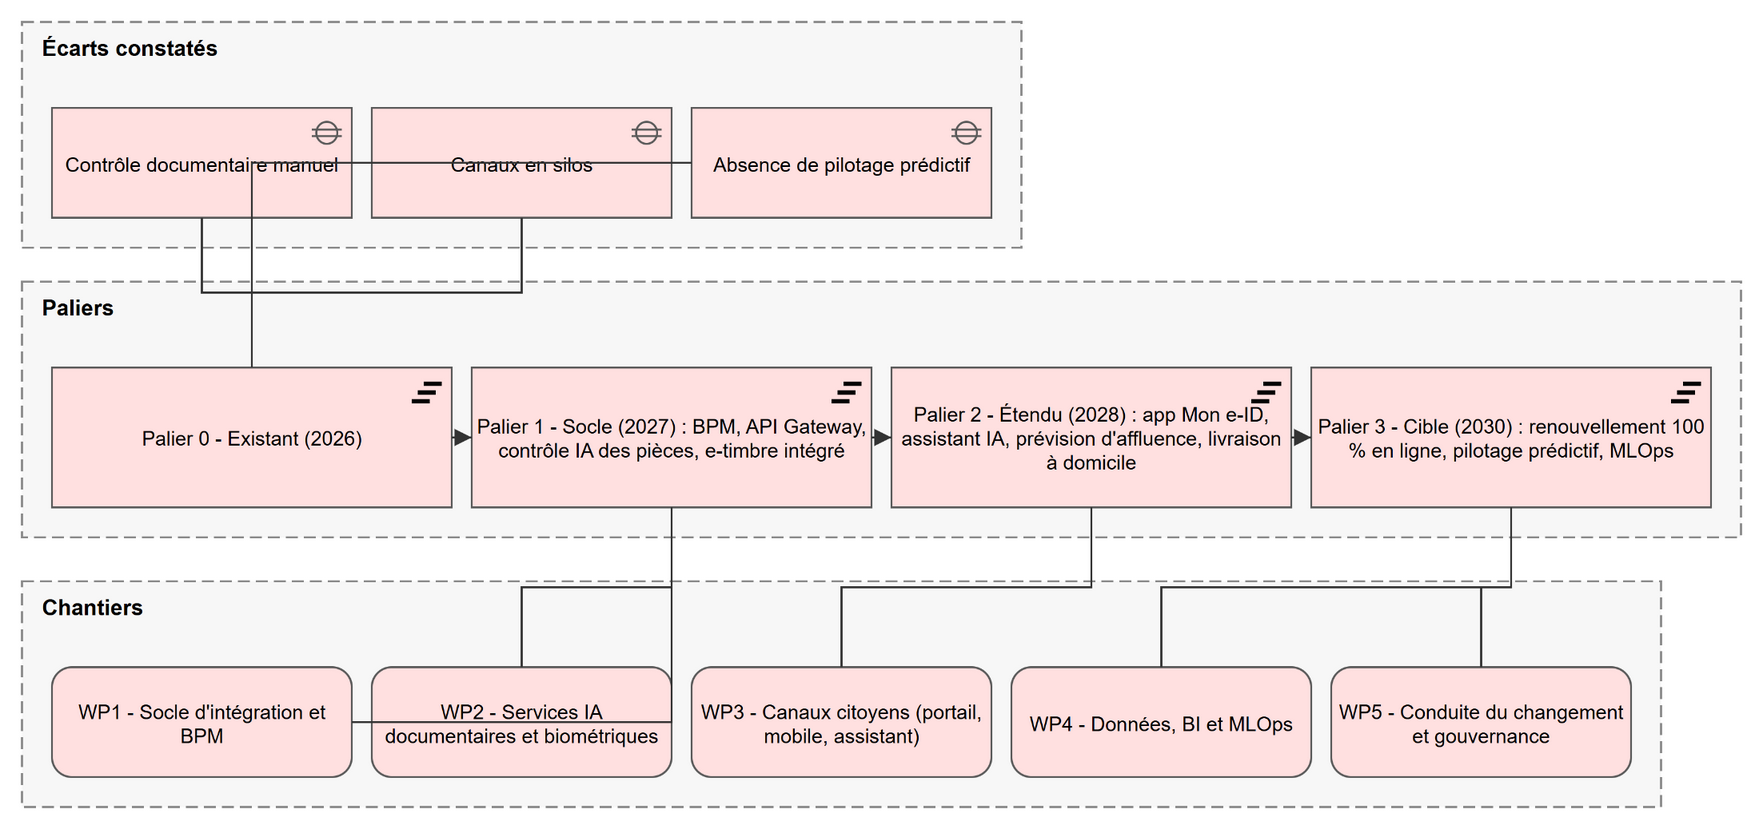
\includegraphics[width=\columnwidth]{archimate/V6_trajectoire.png}
\caption{Trajectoire de migration~: écarts, paliers et chantiers (ArchiMate, couche implémentation et migration).}
\label{fig:trajectoire}
\end{figure}

\subsection{Chantiers et gouvernance}
Cinq chantiers portent la trajectoire~: socle d'intégration et BPM~; services d'IA documentaires et biométriques~; canaux citoyens~; données, BI et MLOps~; conduite du changement et gouvernance. Ce dernier chantier est décisif~: formation des agents des CEDI au nouveau rôle d'accueil, création du métier d'instructeur, communication vers les citoyens, et instauration d'un \emph{comité d'architecture} qui valide chaque évolution au regard des principes d'urbanisation, tient à jour les cartographies et arbitre la dette technique. Un \emph{comité d'éthique de l'IA}, associant la CNDP, examine chaque modèle avant sa mise en service et revoit périodiquement ses indicateurs d'équité.

\subsection{Risques du programme}
\begin{table}[h]
\caption{Principaux risques du programme et parades}
\label{tab:risques}
\centering
\small
\begin{tabularx}{\columnwidth}{XX}
\toprule
\textbf{Risque} & \textbf{Parade} \\
\midrule
Rejet par les agents d'un contrôle automatique perçu comme concurrent & Déploiement en mode assistance d'abord, indicateurs partagés, valorisation du rôle d'instructeur \\
Fracture numérique et exclusion & Maintien du guichet, assistance en centre, assistant vocal multilingue, cas particuliers à domicile \\
Faux rejets du contrôle documentaire & Seuils prudents, instruction humaine systématique de la zone de doute, mesure continue \\
Dépendance à un fournisseur d'IA & Modèles hébergés sur site, formats ouverts, compétences internes \\
Dérive du périmètre & Paliers à valeur mesurable, comité d'architecture, gel des évolutions hors cartographie \\
\bottomrule
\end{tabularx}
\end{table}

\section{Conclusion}
Ce rapport a appliqué la démarche d'urbanisation au périmètre de la carte nationale d'identité électronique. L'étude de l'existant a montré un portail qui a réussi la généralisation du rendez-vous en ligne et une plateforme d'identité numérique souveraine déjà adoptée, mais un processus encore coupé en deux entre le numérique et le guichet, un contrôle des pièces manuel et tardif, et des canaux cloisonnés. La captation de la stratégie a traduit Digital Morocco 2030, la loi 55-19 et les priorités de la DGSN en cinq objectifs mesurables et cinq principes d'urbanisation.

Le système cible décline ces objectifs de manière cohérente sur quatre couches~: un processus P0 reconstruit autour de l'identité numérique, du contrôle documentaire automatique et de l'enrôlement allégé~; un plan d'occupation des sols de trente-deux blocs fonctionnels dont douze nouveaux~; quinze composants applicatifs orchestrés par un moteur de processus et reliés par une passerelle d'API~; une architecture technique en zones, hébergée souverainement, avec une plateforme d'inférence dédiée. Le prototype Bonita du sous-processus de pré-demande a confirmé la faisabilité de l'orchestration et des interfaces. La trajectoire en trois paliers permet de livrer de la valeur dès 2027 tout en maîtrisant les risques humains, techniques et réglementaires.

Deux perspectives prolongent ce travail. La première est l'extension de la démarche aux autres téléservices de la DGSN, pour lesquels le socle d'intégration, le moteur de processus et la plateforme d'IA proposés ici sont directement réutilisables. La seconde est la mesure réelle des gains~: les indicateurs définis dans la cartographie métier devront être instrumentés dès le premier palier afin d'ajuster les seuils de décision des modèles et de documenter, chiffres à l'appui, l'apport de l'intelligence artificielle au service public de l'identité.


\printbibliography

\end{document}
